%% Version 2022-07-08
%% LaTeX-Vorlage für Abschlussarbeiten
%% Erstellt von Nils Potthoff, ab 2020 erneuert und ausgebaut von Simon Lohmann
%% Lehrstuhl Automatisierungstechnik/Informatik Bergische Universität Wuppertal
%%%%%%%%%%%%%%%%%%%%%%%%%%%%%%%%%%%%%%%%%%%%%%%%%%%%%%%%%%%%%%%%%%%%%%%%%%%%%%%%

\chapter{Grundlagen}
	% Hier werden die Grundlagen der Thematik erklärt.
	% Das können z.B. mathematische Grundlagen, Kommunikationsprotokolle oder spezielle Algorithmen sein.
	% Übliches Wissen aus unserer Faktultät wie z.B. die Formel U = R*I kann vorausgesetzt werden.
	%
	% Faustregel: alles, was man selber vorher nicht wusste, aber auch nicht selber entwickelt hat.
	%
	% Hier gilt es aber auch auf Erst- und Zweitgutachter einzugehen.
	% Wenn man weiß, dass einer der beiden ein Thema nicht so genau kennt, sollte es evtl. doch in die Grundlagen.
	%
	% => im Zweifelsfall den Betreuer fragen
	
	% Intro: Wofür? -> Klimaneutralität -> Wärmewende -> Wärmeplanungen -> Tool zur Datenaufbereitung
	% Intro: Was? -> Grob 1), 2), 3)
	Um Klimaneutralität zu erreichen bedarf es einer grundlegenden Transformation des Agrar-, Energie-, Verkehrs- und Wärmesektors. Die Durchführung von Wärmeplanungen stellt dabei ein effektives Instrument für die erfolgreiche Transformation des Wärmesektors dar. Für die Erstellung eines Tools zur systematischen Aufbereitung von Daten für Wärmeplanungen werden in diesem Kapitel die notwendigen Grundlagen ermittelt. Dazu gehören Hintergrundinformationen zur Wärmewende in Deutschland, Wärmeplanungen und Geo-Informations-Systemen. 
	
	% Inhalt: 1) Hintergrundinfo Wärmewende, Bedeutung Wärmeplanungen; 
	In \autoref{sec:Grundlagen:Wärmewende_in_D} wird die Bedeutung von Wärmeplanungen im Kontext der Wärmewende illustriert. Hierfür werden Eckdaten zum Ist-Zustand und zu den politischen Zielvorhaben der Wärmewende in Deutschland beschrieben, exemplarisch die Wärmeplanung eines Fernwärmenetzes in Dänemark vorgestellt und zusätzlich welche Rolle Wärmenetze in zukünftigen Energiesystemen spielen können präsentiert. 
	
	% Inhalt: 2) Wärmeplanungsprinzipien
	Danach wird in \autoref{sec:Grundlagen:Wärmeplanung_Prinzipien} erläutert, welchen Prinzipien Wärmeplanungen folgen. Dazu gehört der Aufbau, der Inhalt und die Herangehensweise bei der Erstellung von Wärmeplanungen. 
	
	% Inhalt: 3) GIS
	Zum Schluss werden in \autoref{sec:Grundlagen:GIS} die Eigenschaften und Funktionen von Geo-Informations-Systemen erklärt, und hilfreiche Informationen geliefert, um mit diesen zu arbeiten.
	
	\section{Wärmewende in Deutschland}
	\label{sec:Grundlagen:Wärmewende_in_D}
		% Intro: Warum schon sec:Grundlagen erläuter
		% Inhalt: 1) Status-Quo, 2) Polit. Ziele, 3) Beispiel, 4) Wärmenetze = Systemdienstleister
		Entscheidend für die Bedeutung des Wärmesektors auf dem Weg zu Klimaneutralität ist dessen Anteil an den gesamten Treibhausgasemissionen (THG-Emissionen). Wie der Status Quo in Deutschland hinsichtlich der geplanten Wärmewende aussieht, welche politischen Zielvorgaben es hierfür gibt und wie eine gelungene Umsetzung aussehen kann, wird in den folgenden Unterkapiteln näher beschrieben.
		
		In \autoref{sec:Grundlagen:Wärmewende_in_D:Ausgangssituation} wird hierfür ein Überblick zur Entwicklung der THG-Emissionen in Deutschland nach Sektoren gegeben, gefolgt von einer Analyse des Gebäudebestandes, des gesamten Wärmeverbrauchs und der Struktur der Wärmeversorgung in Deutschland. 
		
		Danach wird in \autoref{sec:Grundlagen:Wärmewende_in_D:Politische_Zielvorhaben} die aktuelle Zielsetzung der deutschen Bundesregierung bezüglich der Wärmeversorgung beschrieben und die prognostizierten THG-Emissionen bei Erreichen der Ziele mit den Zielen des Pariser Klimaabkommens verglichen.
		
		Daraufhin wird in \autoref{sec:Grundlagen:Wärmewende_in_D:Beispiel_Wärmeplan_Fernwärmenetz} als Muster-Beispiel gelungener Wärmeplanung das Fernwärmenetz in Vojen, Dänemark, vorgestellt. 
		
		Zuletzt wird in \autoref{sec:Grundlagen:Wärmewende_in_D:Wärmenetze_als_Systemdienstleister} die Rolle von Wärmenetzen als Systemdienstleister und deren Funktion in zukunftsfähigen integrierten Energiesystemen beschrieben. 
		
		\subsection{Ausgangssituation}
		\label{sec:Grundlagen:Wärmewende_in_D:Ausgangssituation}
			
			Eine genaue Bilanzierung des Wärmesektors an den THG-Emissionen gestaltet sich aufgrund stark wetterbedingter Schwankungen und ungenauer Datenlage schwierig.  \autoref{fig:UBA_Entwicklung_THG_Emissionen_1990_2019} zeigt die Entwicklung der jährlichen THG-Emissionen für Deutschland vom Referenzjahr 1990 (1249 Mio. t CO2-Äquivalente) bis 2019 inkl. Vorjahres-Schätzung für 2020 (810 Mio. t CO2-Äquivalente) nach Zahlen des Umweltbundesamts. Die Reduktion der gesamten THG-Emissionen von 2019 gegenüber 1990 entspricht ca. 35\%.
			\cite{Umweltbundesamt_Treibhausgasemissionen_Deutschland_seit_1990}
			
			\begin{figure}[h!]
				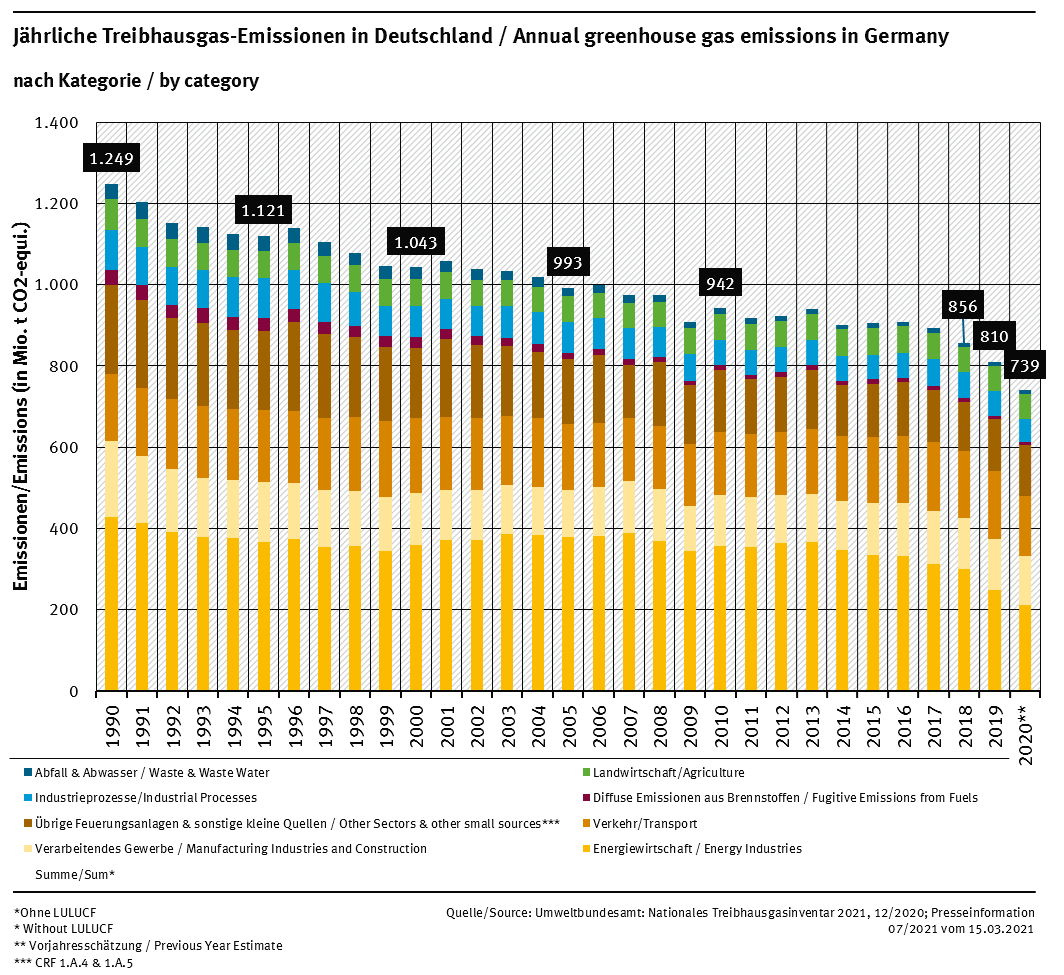
\includegraphics[width=0.7\linewidth]{Medien/own/Umweltbundesamt_Treibhausgasemissionen_Sektoren_1990_bis_2019.png}
				\caption{Entwicklung der jährlichen Treibhausgas-Emissionen in Deutschland\cite{Umweltbundesamt_Treibhausgasemissionen_Deutschland_seit_1990}}
				\label{fig:UBA_Entwicklung_THG_Emissionen_1990_2019}
			\end{figure}
			
			Private Haushalte tragen hauptsächlich durch den Betrieb von Feuerungsanlagen (Anteil von braun) für die Raumwärme- und Warmwasseraufbereitung zur Emission von THG bei.			
			Industrieprozesse (blau) und verarbeitendes Gewerbe (gelb) tragen ebenso einen erheblichen Anteil an Emissionsbelastung bei, wobei diese ebenfalls nur zum Teil auf den anfallenden Wärmebedarf zurückzuführen ist. \cite{Umweltbundesamt_Treibhausgasemissionen_Deutschland_seit_1990}
			
			Die Sektoreneinteilung des Umweltbundesamts in der betrachteten Abbildung lässt somit nur bedingt Rückschlüsse auf den genauen Anteil des Wärmesektors an den gesamten THG-Emissionen zu. Anderen Sektorenaufteilungen der THG-Emissions-Daten des Umweltbundesamts beziffern den Anteil des Gebäudesektors mit ca. 16,9\% im Jahr 1990 (dabei 10,6\% durch Haushalte und 5,3\% durch GHD (ohne Militär und Landwirtschaft)) und ca. 15,2\% im Jahr 2021 (dabei 11,1\% durch Haushalte und 3,9\% durch GHD (ohne Militär und Landwirtschaft)).\cite{Umweltbundesamt_Treibhausgasemissionen_Deutschland}
			
			\todo{CO2-Pfade, 1,5 Grad Ziel, CO2-Budget}
			
			%Notes: Hier eher Methodik was als Ausgangssituation bestimmt werden soll und wie vorgegangen wird! Kurzer Hinweis warum der Wärmesektor so wichtig ist. Und wie dieser analysiert wird. Gebäudebestand, Wärmeverbrauch, Wärmeerzeugung, ...

			\subsubsection{Gebäudebestand in Deutschland}
			\label{sec:Grundlagen:Wärmewende_in_D:Ausgangssituation:Gebäudebestand}
				Die Analyse des Gebäudebstands in Deutschland umfasst in den folgenden Unterkapiteln u.A. eine Beschreibung der Altersstruktur, der Entwicklung des flächenspezifischen Heizbedarfs nach Baualter und der durschnittlichen Wohnfläche pro Person und der Sanierungsraten- und quoten. Zudem enthalten sind Referenzen für die Zusammensetzung eines klimaneutralen Gebäudebestandes und Verweise zu weiterführender Literatur.				
				
				Um den Gebäudebestand näher analysieren zu können bietet sich eine normierte Typologisierung an, damit Gebäude strukturiert anhand ihrer verschiedenen Parameter energetisch bewertet werden können. Eine Einteilung in verschiedene Gebäudetypen nach Größen- und Baualterklassen wird beispielsweise durch das IWU gegeben. \cite{IWU_2015_Wohngebäudetypologie}
				
				\textbf{Altersstruktur des deutschen Gebäudebestands:}\\
				In \autoref{tab:Gebäudematrix_2011} sind die Wohnflächen und Häufigkeiten des deutschen Wohngebeäudebestands nach den Zahlen aus dem Zensus 2011 gegeben. Zu erkennen ist, dass ein Großteil des Gebäude- und Wohnungsbestandes (60\% bzw. 62\%) aus der Zeit vor 1969 stammt. Die aggregierte Wohnfläche der Wohnungen bis 1969 macht dabei einen Anteil von 48\% der gesamten Wohnfläche aus. Dieses ungleiche Verhältnis resultiert aus der in den letzten Jahrzehnten durchschnittlich gestiegenen Wohnfläche/Wohnung \cite{IWU_2015_Wohngebäudetypologie}.
				
				\begin{figure}[H]
					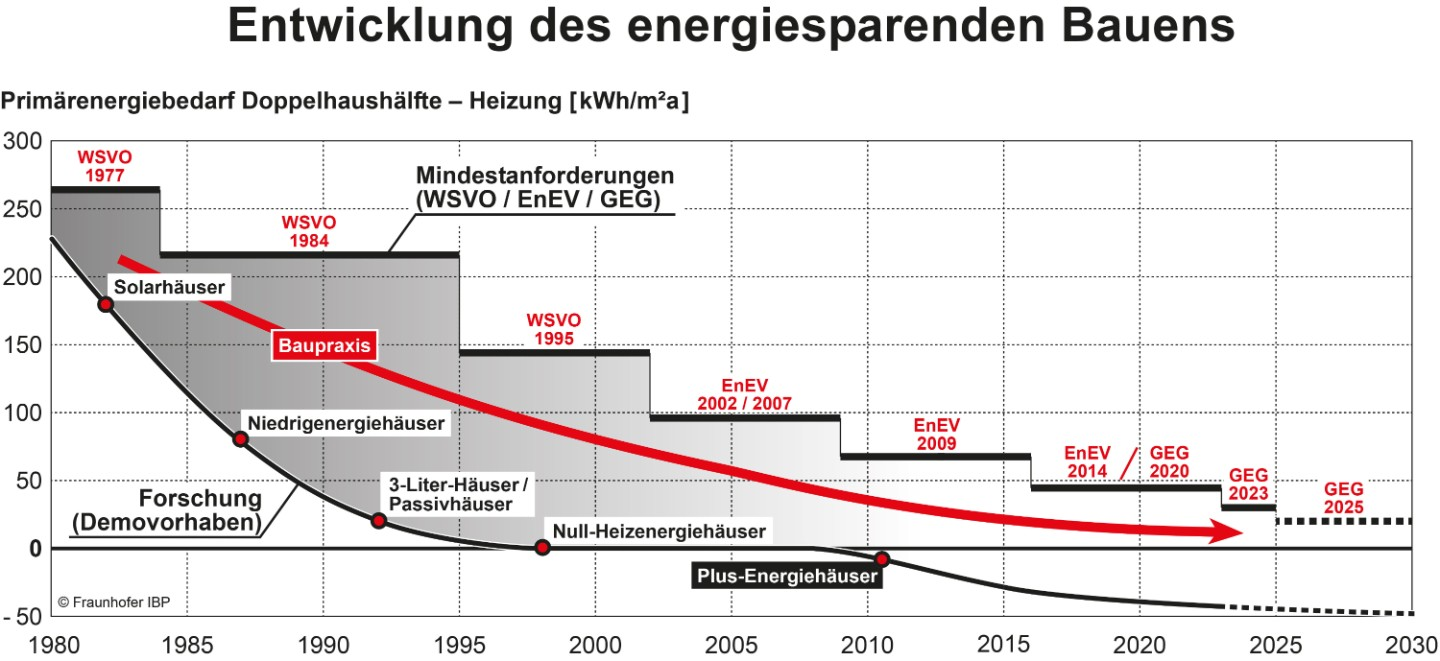
\includegraphics[width=\linewidth]{Medien/own/Fraunhofer_IBP_Entwicklung_des_energiesparenden_Bauens_1980_bis_2020.jpg}
					\caption{Entwicklung des spezifischen Wärmebedarfs von Gebäuden: Regulatorische Mindestanforderungen, Baupraxis und Forschung \cite{IBP_Abb_Entwicklung_Energiesparendes_Bauen}}
					\label{fig:Entwicklung_Energiesparendes_Bauen}
				\end{figure}
			
				\textbf{Entwicklung des flächenspezifischen Heizbedarfs:}\\
				Der typische flächenspeziefische Primärenergiebedarf zum Heizen ist bei Altbauten historisch bedingt deutlich höher als in modernen Gebäuden.  \autoref{fig:Entwicklung_Energiesparendes_Bauen} zeigt exemplarisch die Entwicklung des Primärenergiebedarfs in den letzten Jahrzehnten von 1980 bis 2020 inkl. Prognose bis 2030. Das Fenster von in der Baupraxis üblichen Werte wird begrenzt durch gesetzlich vorgeschriebene Mindeststandards (oberer Treppenverlauf) und Beispiel-Demo-Bauten aus Forschungsprojekten zu energiesparendem Bauen und ambitionierten ökologisch orientierten Hausprojekten (unterer Linie). Der Heizbedarf ist in Neubauten von 1980 bis 2020 in 40 Jahren von über 250 $\frac{kWh}{m^2}$ auf unter 50 $\frac{kWh}{m^2}$ gesunken, was einer Reduktion von über 80\% entspricht. \cite{IBP_Abb_Entwicklung_Energiesparendes_Bauen}\\
				
				\textbf{Entwicklung der genutzten Wohnfläche/Person:}\\
				Das Wuppertal-Institut misst in seiner Transformations-Studie(?) \textit{CO2-neutral bis 2035} der Frage: \textit{"Wie viel Wohnfläche ist genug?"}, eine zentrale Rolle zu. Für die mittelfristige Dekarbonisierung des Gebäudesektors wird hervorgehoben, dass diese Frage mit den anderen beiden Leitfragen: \textit{"Wie energieeffizient sollten Gebäude sein?"}, und: \textit{"Wie sollten die Gebäude beheizt werden?"}, integrativ (statt isoliert voneinander) betrachtet werden muss. 
				
				Die Pro-Kopf-Wohnfläche in Deutschland ist in den letzten Jahrzehten kontinuierlich angestiegen. Anfang der '60er Jahre lag sie noch bei 19 $\frac{m^2}{Person}$, 1990 dann bei 35 $\frac{m^2}{Person}$ und im Jahr 2018 bereits 47 $\frac{m^2}{Person}$, was eine erhebliche Steigerung des Ressourcenbedarfs pro Kopf bedeutet. \cite[S.~93]{Wuppertal_Institut_CO2_neutral_2035} 
				
				\textbf{Sanierungsraten und -quoten:}\\
				Der Heizbedarf von Altbauten lässt sich durch energetische Modernisierungsmaßnahmen wie nachträgliche installierten Dämmungen verbessern, allerdings werden Sanierungsarbeiten nicht zentral erfasst, weder quantitativ noch qualitativ. Laut einer 2018 großangelegt durchgeführten Datenerhebung des IWU betrug die jährliche energetische Sanierungsrate zwischen 0,8\% (im Zeitraum 2005 bis 2008) und 1,0\% (im Zeitraum 2010 bis 2016). 
				\cite[S.~149]{IWU_2018_Wohngebäudebestand_2016}
				
				Die Untersuchung des IWU gibt auch Zahlen zu typischen Dämmquoten von Gebäuden nach IWU-Basis-Geäudetypen (EFH, ZFH, MFH) und an den Mikrozensus angelehnte Baualtersklassen in Hessen an. Die zusammengefassten Ergebnisse für alle Gebäudetypen mit gröberer Zeiteinteilung sind in \autoref{tab:Gebäude_Hessen_Dämmung_2018} gegeben. Zu erkennen ist ein erhebliches theoretisches Potential für nachträgliche Dämmungen.

				\begin{table}[H]
					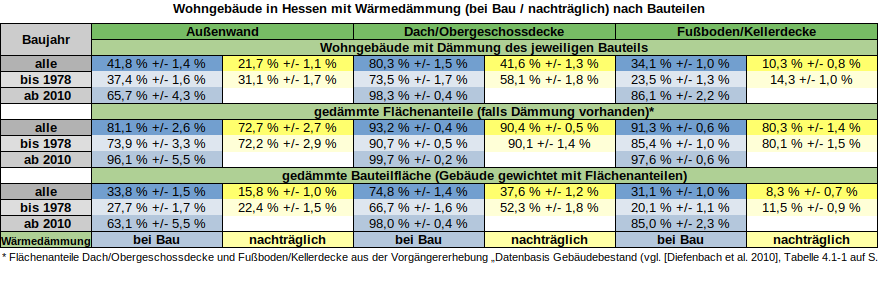
\includegraphics[width=\linewidth]{Medien/tables/IWU_2018_Anteil_Wohngebäude_Hessen_Wärmedämmung_Außen_Dach_Boden.png}
					\caption{Wohngebäude in Hessen mit Wärmedämmung bei Bau bzw. nachträglich durch energetische Modernisierungs-Maßnahmen \cite[S.~108]{IWU_2018_Wohngebäudebestand_2016}, eigene Darstellung}
					\label{tab:Gebäude_Hessen_Dämmung_2018}
				\end{table}

				Weitere relevante Daten zum Gebäude- und Sanierungsstand bietet der Hintergrundbericht \textit{Wohnen und Sanieren - Empirische Wohngebäudedaten seit 2002}. Die zugrundeliegende Studie wurde durchgeführt von der gemeinnützigen GmbH co2online (im Folgenden kurz co2online) und herausgegeben vom Umweltbundesamt im Jahr 2019. In der Studie wird die co2online Datenbank ausgewertet, in welcher seit 2003 Daten aus der Nutzung deren Online-Energieberatungs-Tools erfasst werden. Zum Zeitpunkt der Studie umfasste diese ca. eine Millionen Datensätze. Zudem werden die Daten abgeglichen mit anderen Datensätzen u.A. der Wohngebäude-Bestands-Untersuchung des IWU aus dem Jahr 2016. \cite{Umweltbundesamt_Wohnen_und_Sanieren_2019} 
				
				Ein Überblick zu den Modernisierungsraten nach Bauteil im Vergleich mehrerer Untersuchungen findet sich in \autoref{tab:Umweltbundesamt_Modernisierungsraten_Vgl}. Die Studie von co2online kommt hier zu ähnlichen Ergebnissen wie die Vergleichsstudien. 
				
				\begin{table}[h]
					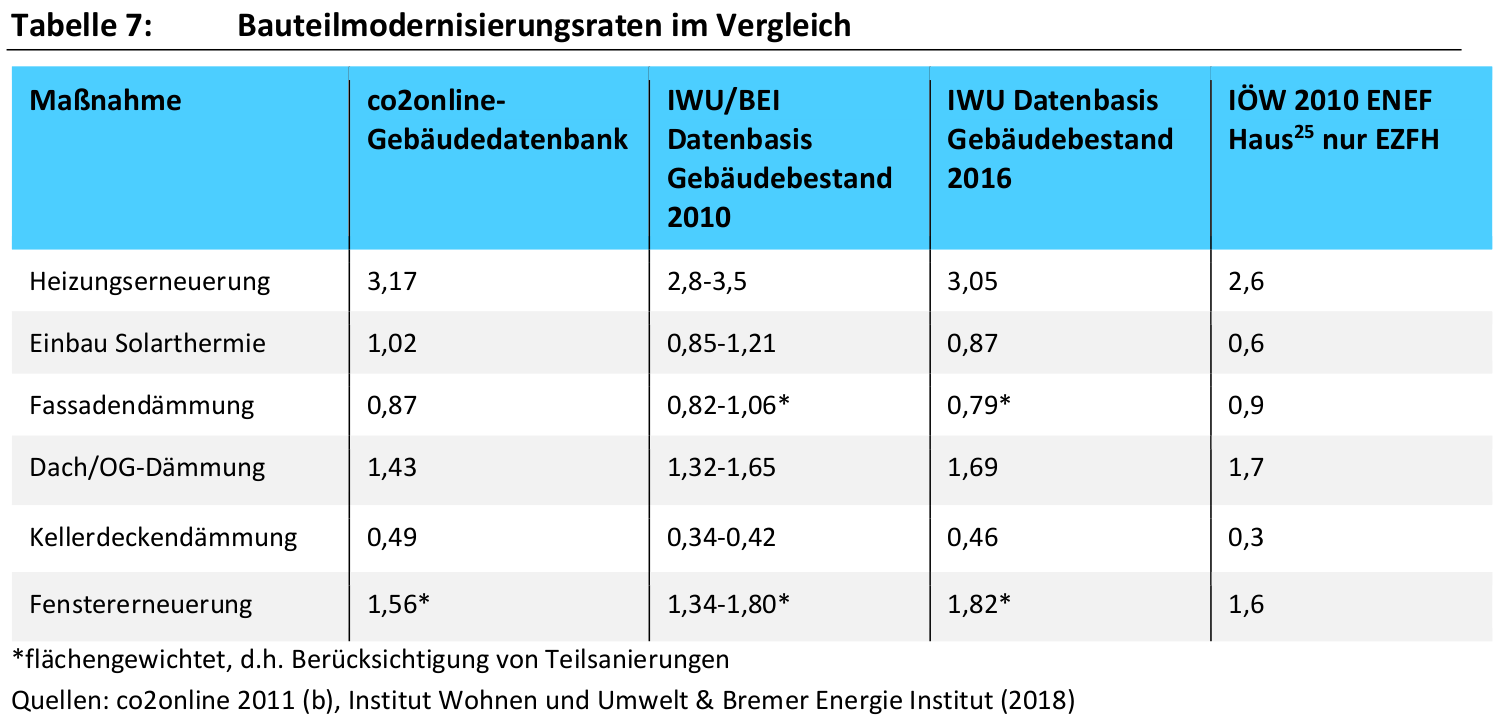
\includegraphics[width=\linewidth]{Medien/tables/Tab_Umweltbundesamt_Bauteilmodernisierungsraten_Vgl_Wohnen_und_Sanieren_2019.png}
					\caption{Bauteilmodernisierungsraten im Vergleich \cite[S.~41]{Umweltbundesamt_Wohnen_und_Sanieren_2019}}
					\label{tab:Umweltbundesamt_Modernisierungsraten_Vgl}
				\end{table}
				
				\textbf{Limitierungen und Hindernisse für Sanierungsarbeiten:}\\
				Das effektive Sanierungspotential wird teils durch regulatorische Restriktionen (Fassaden-Denkmalschutz) oder geometrisch-technisch bedingte Limitierungen begrenzt. Ein weiteres Hindernis kann die Eigentumsstruktur und Kostenverteilung in Mietwohnungen darstellen, da Heizkosten i.d.R. von Bewohnenden gezahlt werden, für Sanierungen aber Wohnungsbesitzende zuständig sind. Hinzu kommen finanzielle und zeitliche Faktoren, dass sich energetische Sanierungen als Langzeitinvestitionen nicht unmittelbar rentieren und teils mit erheblichen Aufwand verbunden sind, was eine Weiternutzung einer Immobilie während Sanierungsarbeiten nicht immer erlaubt. Auf diese und weitere Hindernisse wird auch im Paper Wärmewende im Quartier - Hemmnisse bei der Umsetzung am Beispiel energetischer Quartierskonzepte aus dem Jahr 2016 vom Deutschen Institut für Urbanistik (difu) eingegangen. \cite{difu_2016_waermewende_im_quartier_hemmnisse}\\
				
				\textbf{Eigentumsstruktur des deutschen Wohnungsbestands:}\\
				Die Datenerhebung des Zensus 2011 hat ergeben, dass 43,6\% der Wohnungen in Deutschland von deren Eigentümer*innen bewohnt werden, 51,4\% zu Wohnzwecken vermietet werden und 4,4\% leer stehen, Stand 2011. Die verbleibenden 0,6\% der Wohnungen in Deutschland wurden als Ferien- und Freizeitwohnungen genutzt. \cite[S.~42ff]{Zensus_2011_Ergebnisse}\\
							
				\textbf{Klimaneutraler Gebäudebestand bis 2035:}\\
				Das Wuppertal-Institut kam 2019 zur Einschätzung, dass eine Dekarbonisierung des Gebäudesektors bis 2035 möglich sei, wenn auch mit erheblichen Anstrengungen verbunden. Dafür müsste die jährliche energetische Sanierungsrate auf rund 4 \% gesteigert werden. \cite[S.~95]{Wuppertal_Institut_CO2_neutral_2035}
				
				Als Referenz wie die Beschaffenheit eines klimaneutralen Gebäudebestandes aussehen könnte, kann zudem die Untersuchung \textit{Klimaneutraler Gebäudebestand 2050} des Umweltbundesamtes aus dem Jahr 2015 dienen. In der genannten Studie wird untersucht, wie sich ein Gebäudebestand realisieren ließe, welcher im Jahr 2050 einen nicht-erneuerbaren Primärenergiebedarf von mindestens 80 \% geringer als im Referenzjahr 2008 aufweist. Hierfür wurden verschiedene Zielbilder für 2050 und daraus abgeleitete Transformationspfade entwickelt. Die Festlegung auf das Jahr 2050 entsprang der damaligen politischen Zielsetzung aus dem Jahr 2015. \cite{Umweltbundesamt_Klimaneutraler_Gebäudebestand_2050}\\
								
				\textbf{Weiterführende Literatur zum Gebäudebestand in Deutschland}:\\
				Eine umfangreiche Liste mit weiterführender Literatur und Datenquellen zum Wohngebäudebestand und Gebäude-Energiebilanzen in Deutschland findet sich im Hintergrundbericht \textit{Wohnen und Sanieren - Empirische Wohngebäudedaten seit 2002} des Umweltbundesamtes. \cite[S.~59ff]{Umweltbundesamt_Wohnen_und_Sanieren_2019}
						
			\subsubsection{Wärmeverbrauch in Deutschland}
			
				Ein guter Indikator für die Bedeutung des Wärmesektors sowohl hinsichtlich Klimaneutralität als auch Ressourcenunabhängigkeit ist dessen Anteil am Endenergieverbrauch.

				Der Anteil von Wärme und Kälte (ohne Strom) beträgt in etwa die Hälfte des gesamten Endenergieverbrauch in Deutschland. \autoref{fig:Endenergieverbrauch_D_2019} zeigt exemplarisch die Anteile für Wärme und Kälte (ohne Strom), Verkehr (ohne Strom und int. Flugverkehr) und Nettostromverbrauch am gesamten Endenergieverbrauch von 2391 TWh im Jahr 2019 nach Zahlen der Agentur für Erneuerbare Energien e.V.. \cite{AEE_abb_Endenergieverbrauch_D_2019_Strom_Wärme_Verkehr} 
				
				\begin{figure}[h]
					\centering
					\subfloat[Subfigure 1 list of figures text][Anteil des Wärmesektors am Endenergieverbrauch in Deutschland 2019 \cite{AEE_abb_Endenergieverbrauch_D_2019_Strom_Wärme_Verkehr}]{
						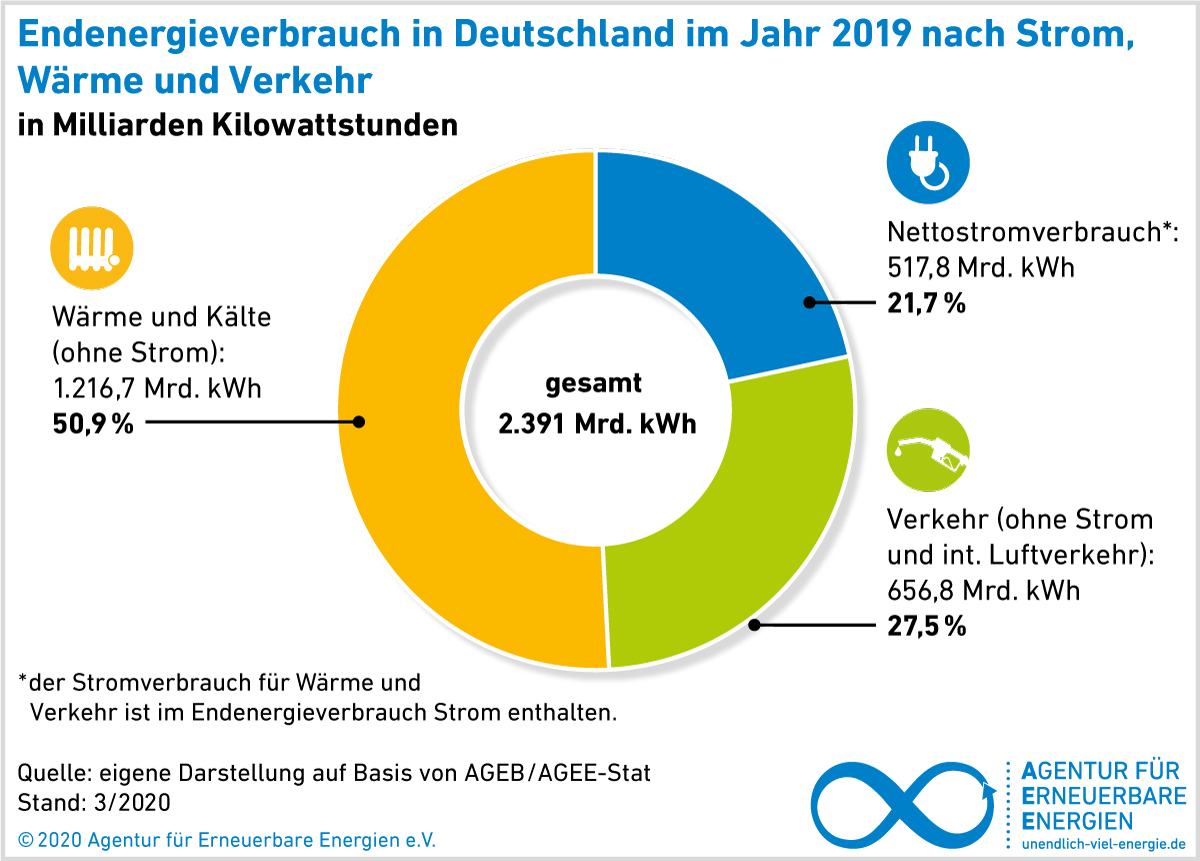
\includegraphics[width=0.5\textwidth]{Medien/own/AEE_Endenergieverbrauch_Strom_Waerme_Kraftstoffe_2019.jpg}
						\label{fig:Endenergieverbrauch_D_2019}}
					\subfloat[Subfigure 2 list of figures text][Aufteilung des Wärmeverbrauchs auf Raumwärme, Prozesswärme und weitere.\cite{Umweltbundesamt_Energieverbrauch_Wärme}]{
						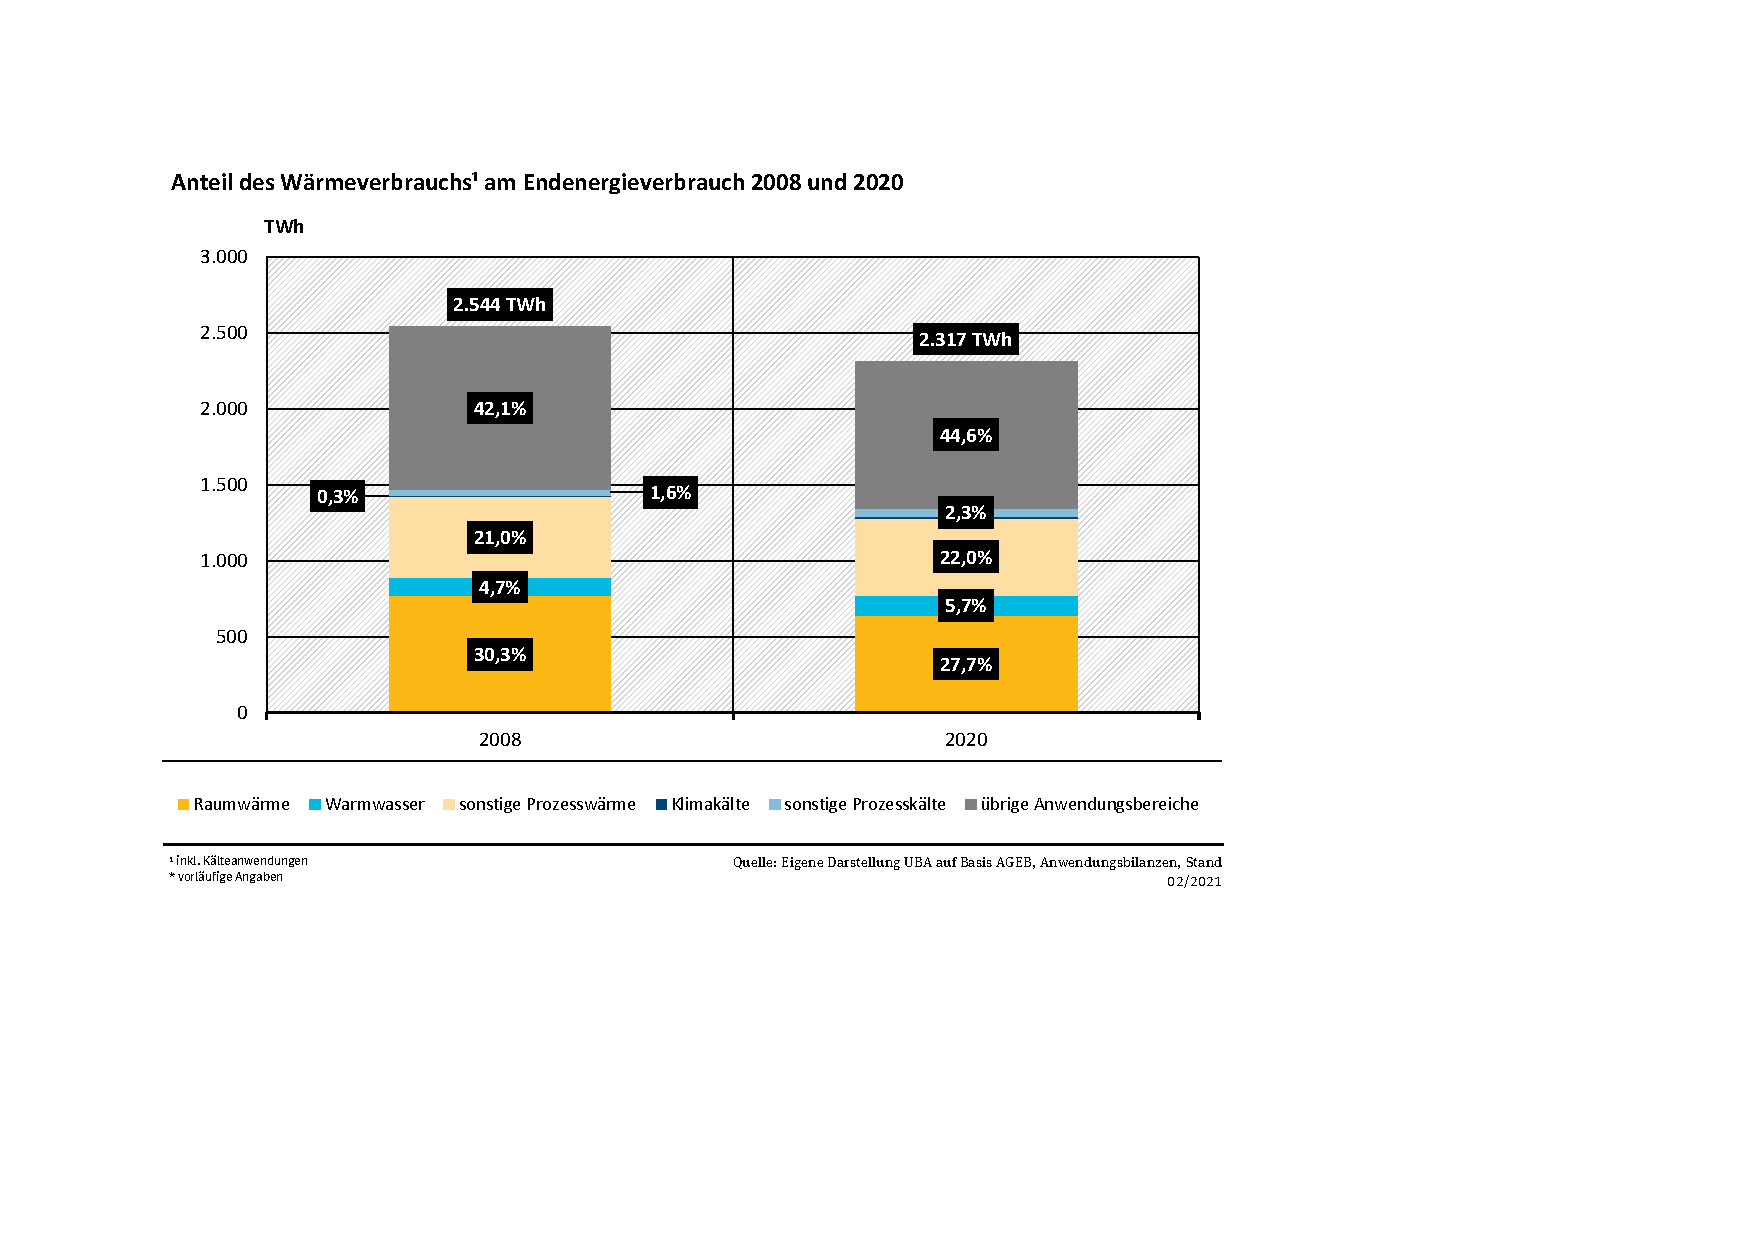
\includegraphics[width=0.5\textwidth]{Medien/own/Anteil_Waermeverbrauch_Endenergieverbrauch_Umweltbundesamt_2022-12-19.pdf}
						\label{fig:Endenergieverbrauch_D_2008_2020}}
					\caption{Wärmeverbrauchs-Anteil am Endenergieverbrauch, aufgeteilt in Raum- und Prozesswärme}
				\end{figure}
				
% OLD DEPRECATED now with usepackage[...]{subfig}
%				\begin{figure}[H]
%					\begin{subfigure}{0.5\linewidth}
%						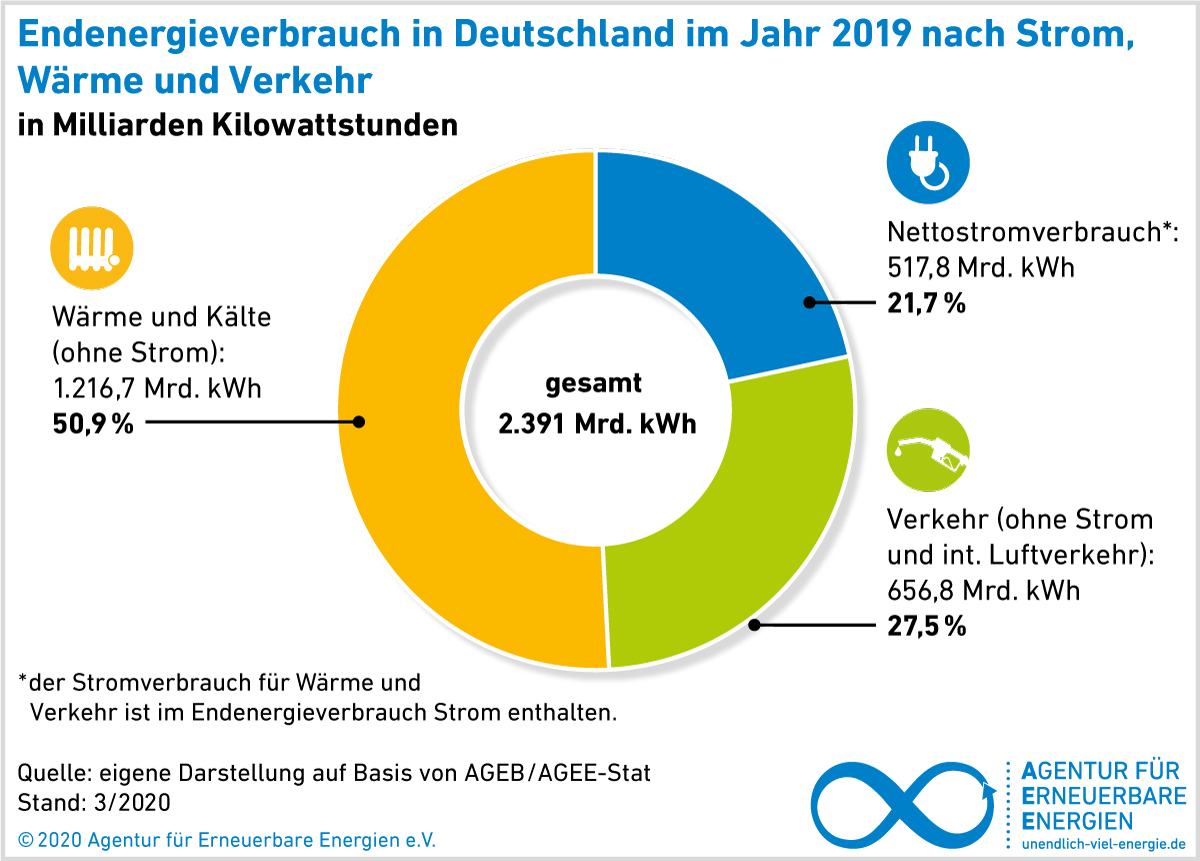
\includegraphics[width=\linewidth]{Medien/own/AEE_Endenergieverbrauch_Strom_Waerme_Kraftstoffe_2019.jpg}
%						\caption{Anteil des Wärmesektors am Endenergieverbrauch in Deutschland 2019 \cite{AEE_abb_Endenergieverbrauch_D_2019_Strom_Wärme_Verkehr}}
%						\label{fig:Endenergieverbrauch_D_2019}
%					\end{subfigure}
%					\begin{subfigure}{0.5\linewidth}
%						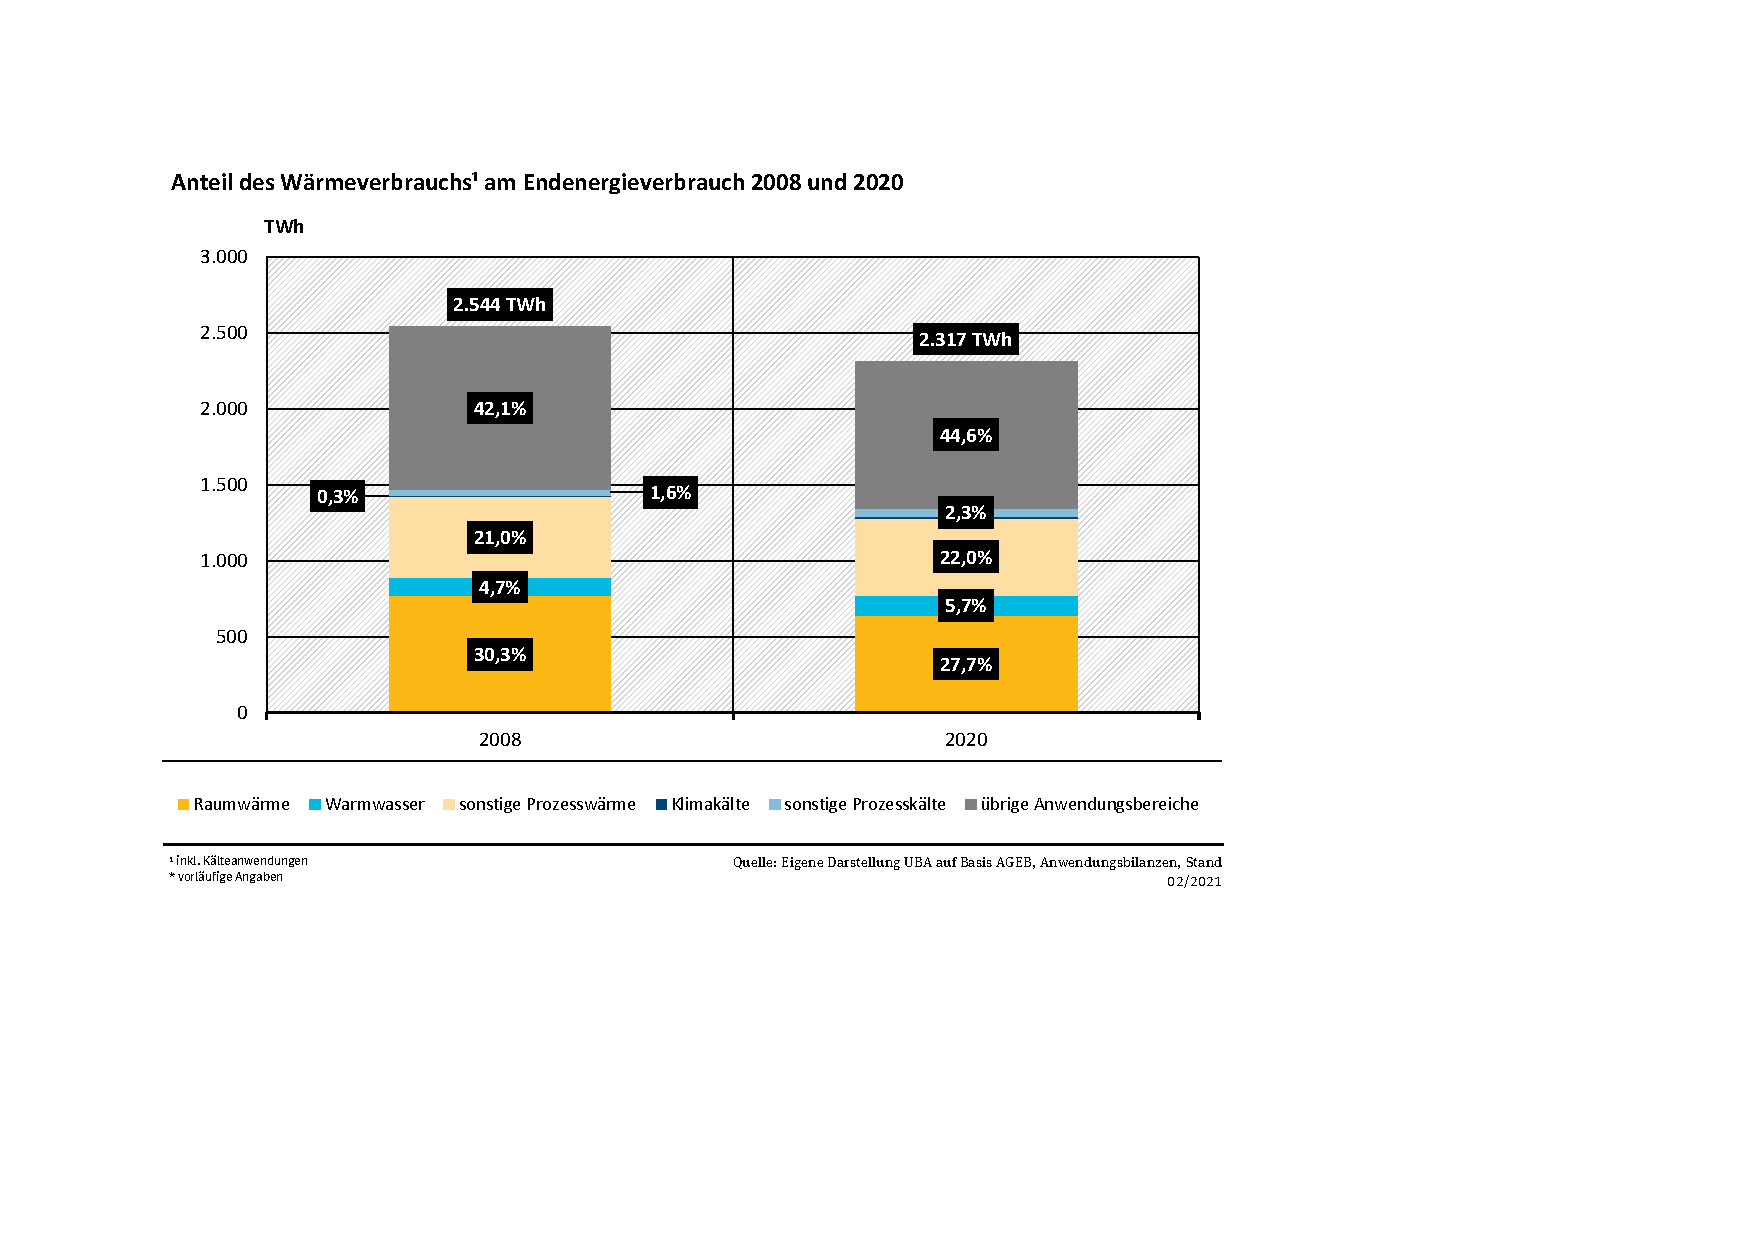
\includegraphics[width=\linewidth]{Medien/own/Anteil_Waermeverbrauch_Endenergieverbrauch_Umweltbundesamt_2022-12-19.pdf}
%						\caption{Aufteilung des Wärmeverbrauchs auf Raumwärme, Prozesswärme und weitere.\cite{Umweltbundesamt_Energieverbrauch_Wärme}}
%						\label{fig:Endenergieverbrauch_D_2008_2020}
%					\end{subfigure}
%				\end{figure}

				In etwa die Hälfte des Wärmebedarfs in Deutschland ging im Jahr 2020 auf die Erzeugung von Raumwärme zurück, etwa 10\% auf die Erwärmung von Warmwasser und der große Rest auf die Erzeugung von Prozesswärme. Die Anteile für Raumwärme, Prozesswärme und Warmwasser am Endenergieverbrauch werden exemplarisch in \autoref{fig:Endenergieverbrauch_D_2008_2020} vergleichsweise für die Jahre 2008 und 2020 gezeigt. Darstellung Zahlen stammen vom Umweltbundesamt. \cite{Umweltbundesamt_Energieverbrauch_Wärme}  

				Hervorzuheben ist, dass es sich bei beiden Graphiken um den Endenergieverbrauch handelt. Der Verbrauch fossiler Primärenergieträger ist ohne Berücksichtigung deren unterschiedlicher Anteile an der Erzeugung von Wärme, Strom und Mobilität neben Erneuerbaren Energien sowie der unterschiedlichen Wirkungsgrade konventioneller thermischer fossiler-Energieträger-betriebener Kraftwerke im Strom- und Verbrennungs-Motor-Antriebe im Verkehrssektor nicht direkt ableitbar. 
				
				Der Primärenergiebedarf für Deutschland betrug laut Datenreport Umwelt, Energie und Mobilität des Statistischen Bundesamtes aus dem Jahr 2021 insgesamt 13.170 PJ (ca 3.658 TWh) im Jahr 2018. Vom Gesamtprimärenergiebedarf entfielen dabei ca. 39 \% auf die Industrie, 33 \% auf private Haushalte und 26 \% auf die Dienstleistungsbereiche. Der Primärenergiebedarf privater Haushalte teilt sich wiederum zu knapp zwei Dritteln (64 \%) auf den Bereich Wohnen und etwa ein Drittel (36 \%) auf den Bereich Mobilität (motorisierter Individualverkehr) auf. Der Energieverbrauch privater Haushalte im Bereich Wohnen nach Energieträger im Jahr 2018 wird hier gesamt mit 2703 PJ (ca. 751 TWh) angegeben, wovon der Großteil (ca. 82,8 \%) für die Erzeugung von Wärme aufgewendet wird die verbleibenden 17,2 \% direkt in Form von Strom genutzt werden. \cite{Destatis_Datenreport_2021_Umwelt_Energie_Mobilitaet}
				
				Eine direkter Vergleich der verschiedenen Zahlen und eine genaue Bilanzierung des Energieverbrauchs oder der CO2-Emissionen des Wärmesektors aufgeteilt nach Sektoren gestaltet sich schwierig. Die gefundenen Daten stammen teils aus anderen Jahren, folgen unterschiedlichen Aufteilungen (i.d.R. nach Sektoren, Energieträger oder Funktion) oder sind älter als 18 Jahre.  
				
				Für das Jahr 2004 findet sich eine simultanen Aufteilung des Endenergieverbrauchs nach Sektoren (Industrie, GHD, Haushalte, Verkehr) und Funktionen (u.A. Raumwärme, Warmwasser, Prozesswärme) in dem im Jahr 2007 veröffentlichten Sachstandsbericht Wohnen, Energie, Mobolität des Umweltbundesamtes. Im Jahr 2004 betrug der Anteil von Haushalten 46,7 \%, von der Industrie 33,1 \% und von GHD 20,0 \% am gesamten Wärmeverbrauch. \cite[S.~27]{UBA_2007_Nachhaltige_Waermeversorgung}
				
				Aktuellere Zahlen zu den energiebedingten CO2-Emissionen zum Heizen (temperaturbereinigt) in privaten Haushalten liefert das Statistische Bundesamt in seinen umweltökonomischen Gesamtrechnungen. Das Heizen privater Haushalte in Deutschland trug nach diesen Rechnungen im Jahr 2020 mit 144 Mio. t CO2 den größten Teil (72,5 \%) der in privaten Haushalten zum Wohnen anfallenden Emissionen von insgesamt 199 Mio. t CO2 bei und verursachte damit in etwa 18,4\% der gesamten im Jahr 2020 in Deutschland angefallenen THG-Emissionen von 825 Mio. t CO2 gemäß Kyoto-Protokoll. \cite[S.~20]{destatis_2022_umweltoekonomische_gesamtrechnung_haushalte_umwelt} \cite[S.~16]{destatis_2022_umweltoekonomische_gesamtrechnung_anthropogene_luftemissionen}
				
				Das Statistische Bundesamt ermittelt diese CO2-Emissions-Zahlen mit Modellrechnungen in einem Bottom-Up-Verfahren anhand von Gebäude- und Wohnungsdaten aus dem Mikrozensus und flächenspezifischen Heizenergie-Verbräuchen bei Heizöl, Gas und Fernwärme gemäß Heizspiegel der gemeinnützigen Beratungsgesellschaft co2online mbH sowie anderen Quellen und Schätzungen. Die Daten sind zudem temperaturbereinigt durch Verrechnung der Heizgradtage. \cite{destatis_2020_umweltökonomische_gesamtrechnung_haushalte_umwelt_methodik}
				
				Das UBA kommt zum Vergleich in seinen Berechnungen zu einem Ergebnis von 91 Mio t CO2-Äq. energiebedingte Emissionen für Haushalte in Deutschland im Jahr 2020. \cite{uba_2022_energiebedingte_emissionen_brennstoffeinsätze_in_D_1990_2020}

			
			\subsubsection{Wärmeerzeugung in Deutschland}
				
				Die Wärmeerzeugung in Deutschland wird noch zum größten Teil mit fossilen Brennstoffen bewerkstelligt, wobei Gas etwa die Hälfte und Öl noch ca. ein Siebtel der gesamten Versorgung ausmacht. Der Anteil der Erneuerbaren an der Wärmeerzeugung betrug 1990 noch einen verschwindend geringen Anteil von ca. 2 Prozet was sich auch bis ca. 1996 nicht änderte. Erst ab 1996 stieg der Anteil Erneuerbarer in einem Zeitraum von etwa 2 Jahren, um 2 Prozent an, stagnierte dann wieder etwas bis 2005 als er ca 5 Prozent betrug. Ab 2005 stieg der EE-Anteil in annäherend linearer Progression auf 14 Prozent im Jahr 2012, was einer Wachstumsrate von etwa 1,29 Prozent pro Jahr entspricht. Danach stagnierte das Wachstum wieder bis 2017, als der EE-Anteil wieder einen kurzen Anstieg auf etwa 15 Prozent im Jahr 2018 stieg und dann schleichend auf 16,5 Prozent im Jahr 2021 stieg. Das bedeutet, dass auch 2021 noch lediglich ein Sechstel der Wärme durch EE erzeugt wurde und der Zuwachs der EE im Wärmesektor selbst in bis dato größten Wachstumsphasen kaum mehr als ein Prozent pro Jahr betrug. \cite{Umweltbundesamt_Energieverbrauch_Wärme} \cite{Umweltbundesamt_Abb_Entwicklung_Anteil_EE_Wärme_Kälte}

% Zweiter Versuch jetzt mit Unterlisting in Abbildungsverzeichnis mit usepackage[lofdepth,lotdepth]{subfig}
% Dafür Unterkante auf einer Höhe
				\begin{figure}[h]
					\centering
					\subfloat[Subfigure 1 list of figures text][Entwicklung des Anteils Erneuerbarer Energien nach Sektor Strom, Wärme und Verkehr, 1990 bis 2021 \cite{Umweltbundesamt_Abb_Entwicklung_EE_Strom_Wärme_Verkehr_1990_2021}]{
						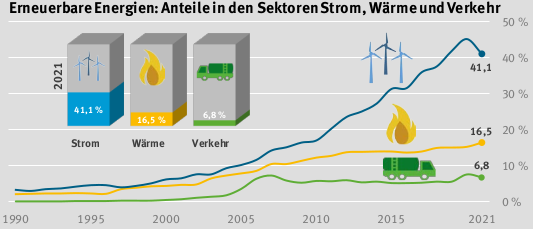
\includegraphics[width=0.5\textwidth]{Medien/own/ee_anteile_in_den_sektoren_strom_waerme_und_verkehr_Umweltundesamt_1990_bis_2021.png}
						\label{fig:Entwicklung_EE_Anteil_nach_Sektoren}}
					\subfloat[Subfigure 2 list of figures text][Entwicklung des Gesamt-Wärmeverbrauchs nach Energieträger von 2008 bis 2021 \cite{Umweltbundesamt_Abb_Wärmeverbrauch_Energieträger_2008_2020}]{
						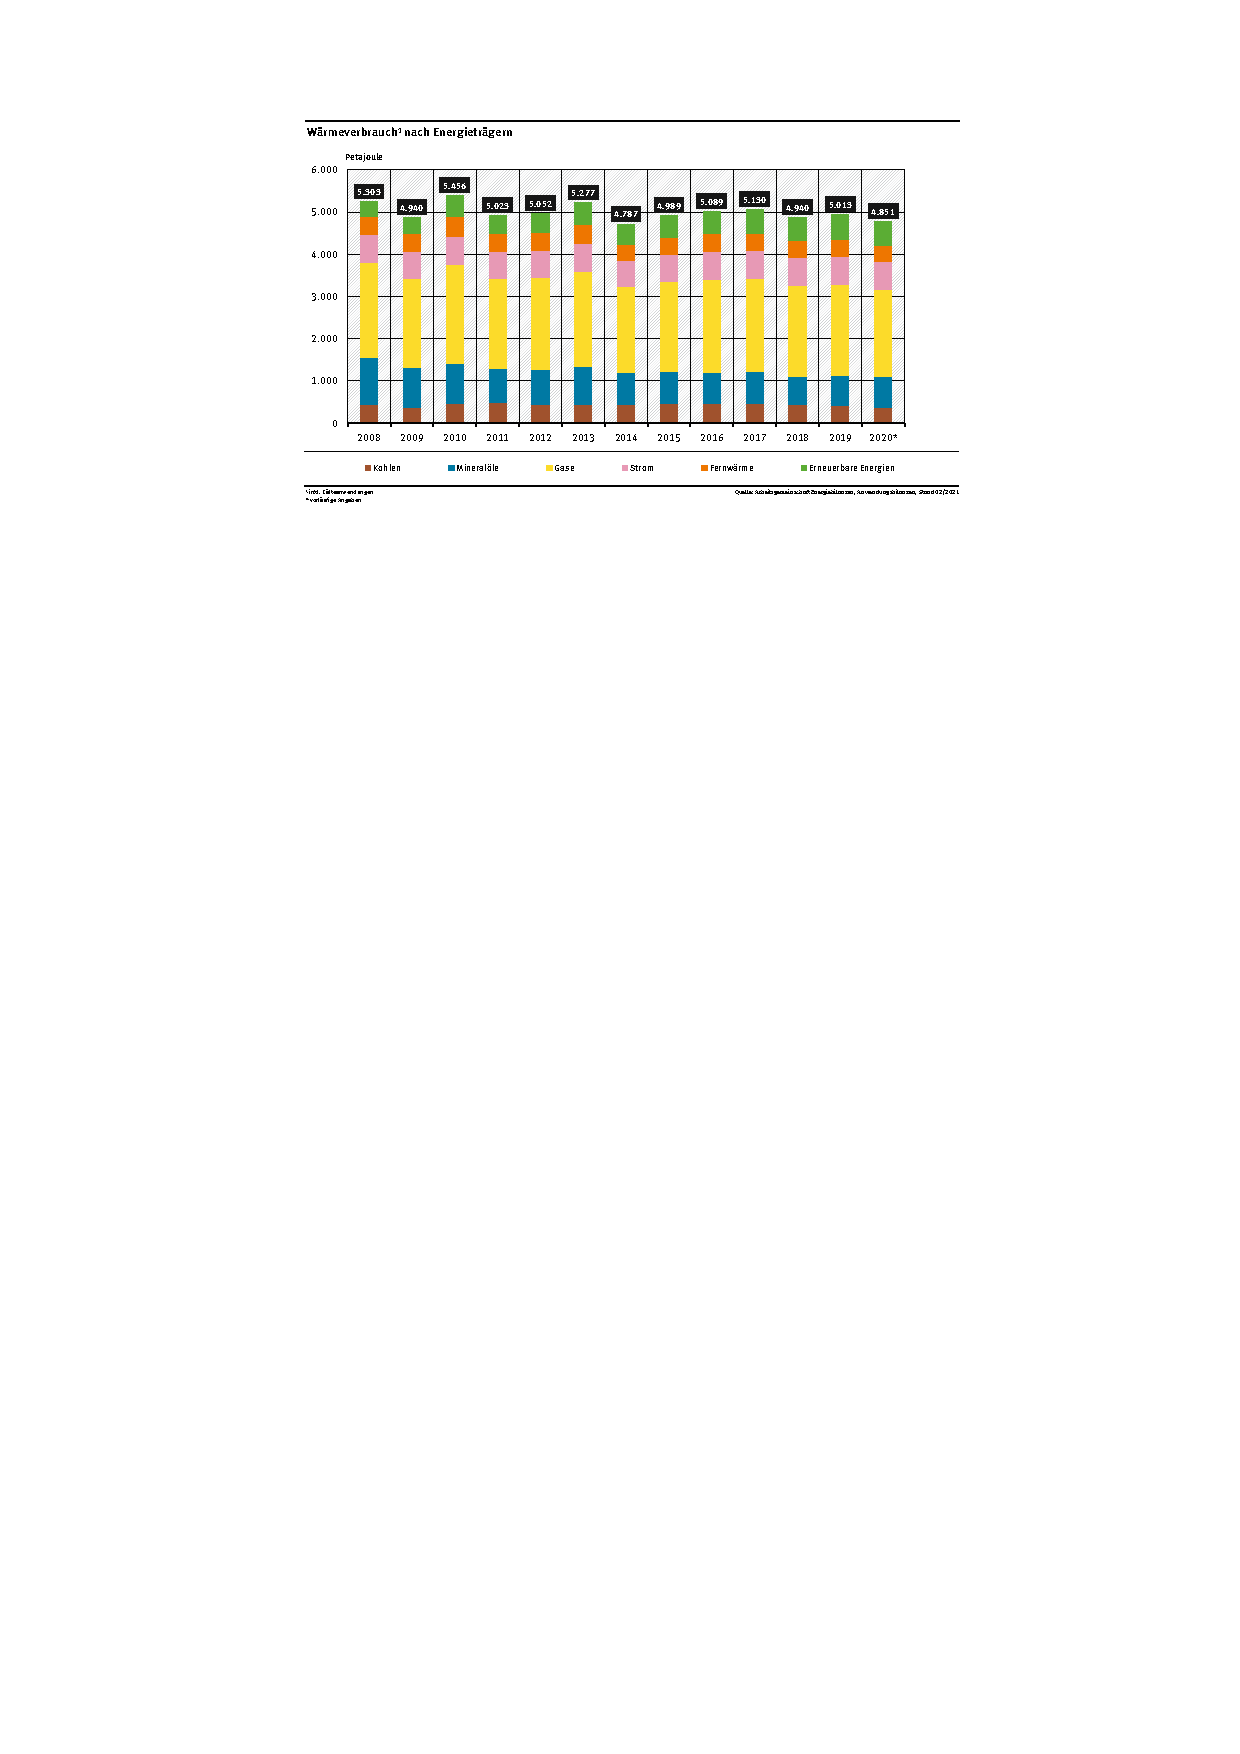
\includegraphics[width=0.5\textwidth]{Medien/own/Wärmeverbrauch_nach_Energieträgern_Umweltbundesamt_2022-12-19.pdf}
						\label{fig:Entwicklung_Wärmeverbrauch_nach_Energieträgern}}
					\caption{Entwicklung des Anteils Erneuerbarer Energien im Wärmesektor in Deutschland}
				\end{figure}


% Erster Versuch: Broken durch usepackage[lofdepth,lotdepth]{subfig} 
%				\begin{figure}[H]
%					\begin{subfigure}{0.45\linewidth}
%						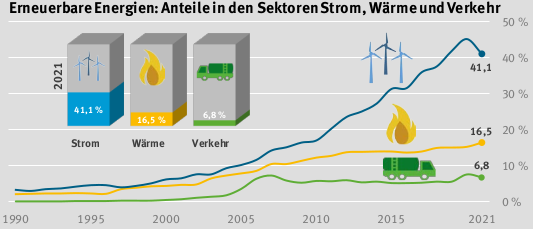
\includegraphics[width=\linewidth]{Medien/own/ee_anteile_in_den_sektoren_strom_waerme_und_verkehr_Umweltundesamt_1990_bis_2021.png}
%						\caption{Entwicklung Anteil Erneuerbarer Energien nach Sektoren Strom, Wärme und Verkehr von 1990 bis 2021  \cite{Umweltbundesamt_Abb_Entwicklung_EE_Strom_Wärme_Verkehr_1990_2021}}
%						\label{fig:Entwicklung_EE_Anteil_nach_Sektoren}
%					\end{subfigure}
%					\begin{subfigure}{0.55\linewidth}
%						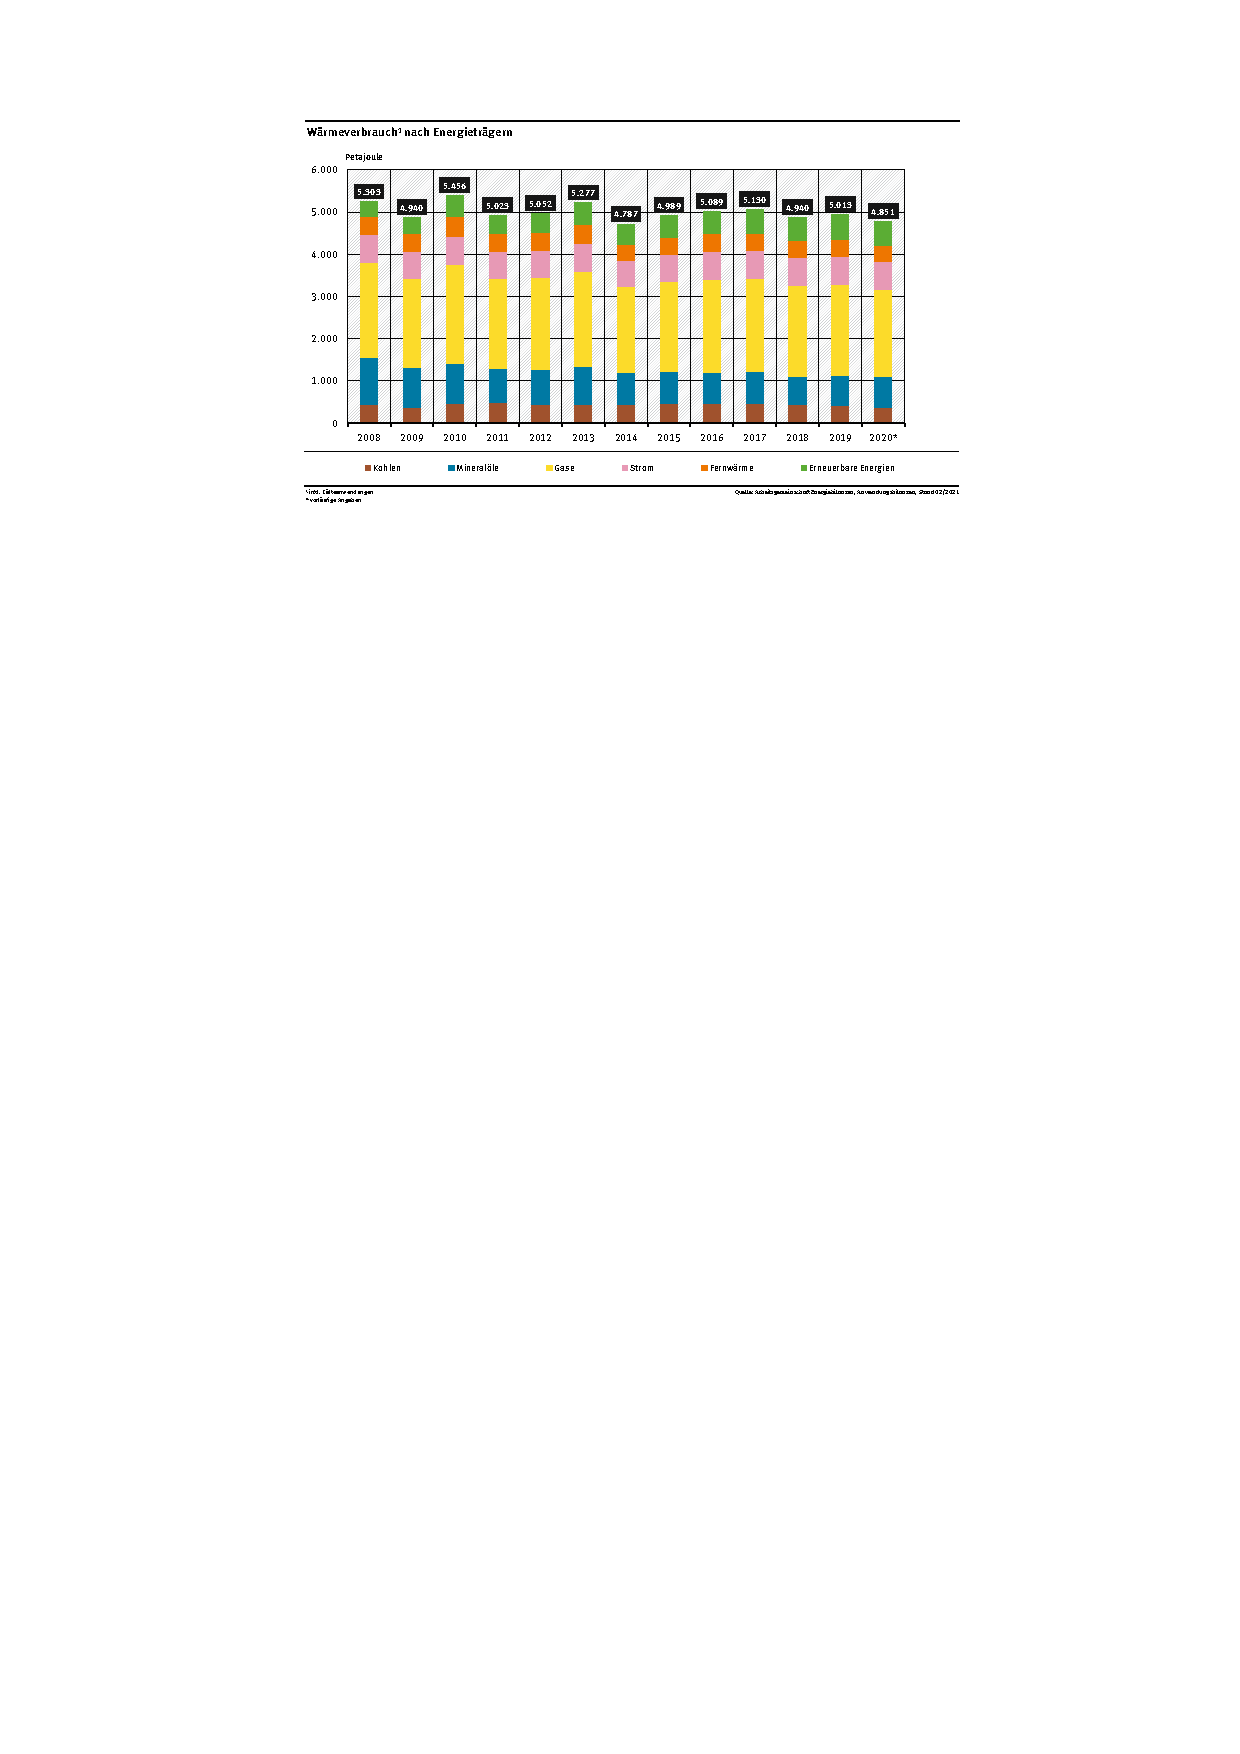
\includegraphics[width=\linewidth]{Medien/own/Wärmeverbrauch_nach_Energieträgern_Umweltbundesamt_2022-12-19.pdf}
%						\caption{Entwicklung Wärmeverbrauch nach Energieträger von 2008 bis 2021 \cite{Umweltbundesamt_Abb_Wärmeverbrauch_Energieträger_2008_2020}}
%						\label{fig:Entwicklung_Wärmeverbrauch_nach_Energieträgern}
%					\end{subfigure}
%					\caption{Entwicklung des Anteils Erneuerbarer im Wärmesektor in Deutschland}
%				\end{figure}
				
				In \autoref{fig:Entwicklung_EE_Anteil_nach_Sektoren} ist zum Vergleich die Entwicklung des relativen Anteils Erneuerbarer im Wärme-, Strom- und Verkehrssektor von 1990 bis 2021 dargestellt nach Zahlen des Umweltbundesamt.
				
				Die Entwicklung der Anteile der verschiedenen Energieträger inklusive Fernwärmenetzen an der Wärmeerzeugung respektive des Verbrauchs von 2008 bis 2019 mit damaliger Prognose für 2020 nach Zahlen der Arbeitsgemeinschaft Energiebilanzen ist in \autoref{fig:Entwicklung_Wärmeverbrauch_nach_Energieträgern} gezeigt. Zu erkennen ist, dass sich sowohl der Gesamtverbrauch als auch die kalorische relative Zusammensetzung nach genutzten Energieträgern für die Wärmeerzeugung in den letzten 15 Jahren nur geringfügig geändert hat. Gleiches gilt für den geringen Anteil von Fernwärme-Netzen an der Wärmeversorgung. 2019 betrug der Fernwärme-Anteil ca. 8 Prozent, der direkte EE-Anteil ca. 12 Prozent der stromgewonnene Anteil ca. 13 Prozent an der Wärmeversorgung. Der durschnittliche Anteil an EE im Stromsektor betrug 2021 ca. 41,4 Prozent und an der Fernwärme-Gewinnung ca. 21,7 Prozent. Auch in Fernwärmenetzen wurde 2021 noch etwa 43,6 Prozent der Wärme aus Gas gewonnen, womit die Zahlen von der Arbeitsgemeinschaft Energiebilanzen und vom Umweltbundesamt zu ähnlichen Ergebnissen kommen.
				
				
		\subsection{Politische Zielvorgaben}
		\label{sec:Grundlagen:Wärmewende_in_D:Politische_Zielvorhaben}
			% Intro 
			Für die Wärmewende relevante Zielvorgaben der Bundesregierung sind in mehreren Gesetzen, Verordnungen und Richtlinien festgelegt. Am bedeutendsten für die Klimaziele der Bundesregierung auf Bundesebene im Allgemeinen und für den Wärmesektor ist das Klimaschutzgesetz (KSG). Ebenfalls von hoher Relevanz für die Wärmewende ist das Gebäudeenergiegesetz (GEG). Ein grober Überblick über den Inhalt der erwähnten Gesetze wird in den folgenden zwei Unterkapiteln gegeben. Zudem werden die Klimaziele des KSG mit dem 1,5-Grad-Ziel des ebenfalls von der Bundesregierung mit unterzeichneten internationalen Pariser Klima-Abkommens verglichen. 
			
			% Ausschluss
			Gesetze, Verordnungen und Richtlinien zur praktischen Umsetzung der Wärmewende, wie planungsrechtliche, baurechtliche, umweltrechtliche oder andere Regulationen sowie Förderungsbestimmungen werden in diesem Kapitel nicht weiter betrachtet.
			% Kraft-Wärme-Kopplungs-Gesetz (KWK-G), die Maßnahmen im Fit-for-55 Paket und die Energieeffizienzrichtlinie 			
			
			\subsubsection{Klimaziele des Klimaschutzgesetzes (KSG)}
			
				% Klimaschutzgesetz KSG
				Im novellierten KSG von 2021 hat die deutsche Bundesregierung ihre Klimaziele nach oben angepasst mit den Zielvorgaben nunmehr bis 2045 (statt 2050) Klimaneutralität zu erreichen und die THG-Emissionen bis 2030 um min. 65 \% (statt 55 \%) und bis 2040 um min. 88 \% gegenüber 1990 zu verringern.\cite{web_gesetze_ksg_info}\cite{web_gesetze_ksg}
				
				% Abgleich KSG und Pariser Klimaabkommen
				Aus den im KSG angegebenen sektorspezifischen THG-Reduktionspfaden bis 2030 (mit Ausnahme der Energiewirtschaft) und den prozentualen Reduktionszielen bis 2040 und Annahmen zum zukünftigen Einbezug natürlicher CO2-Senken und der weiteren Entwicklung der nicht CO2-THG-Emissionen lässt sich ein CO2-Budget ableiten. 
				
				Der Sachverständigen-Rat für Umweltfragen (SRU) listet in seiner Stellungnahme zur KSG-Novellierung verschiedene Untersuchungen zu Berechnungen des aus dem KSG resultierenden CO2 Budgets, die auf Ergebnisse zwischen 6,4 und 7,4 Gt CO2-Emissionen ab dem Jahr 2022 kamen.\cite[S.~14]{SRU_Stellungnahme_CO2_Budget_2022} Vergleich: \cite[S.~12]{mcc_2022_ist_deutschland_auf_1_5_grad_pfad}, \cite[S.~11]{zbw_2022_pariskompatible_emissionspfade_bsp_eu}, kommt in der aktualisierten Version von 2022 sogar auf ein aus dem KSG abgeleitetes CO2-Budget von 7,9 Gt CO2-Emissionen, \cite{knoe_2022_mit_grüner_marktwirtschaft_klima_retten} German Zero leitet aus dem KSG einen Beitrag zur globalen Erderwärmung ab, der einer Erwärmung von 1,8°C entspräche. \cite[S.~37]{germanzero_2022_gesetztespaket_1_5_grad}

				% Resumé
				Selbst unter Einhaltung der KSG-Ziele würde die deutsche Bundesregierung demnach das vereinbarte 1,5°C-Ziel des Pariser Klimaabkommens sehr wahrscheinlich verfehlen. Ein erheblicher Fortschritt gegenüber früheren Klimaschutz-Ambitionen stellt das KSG dennoch dar, da es zumindest einem Beitrag entspricht, der die Erderwärmung auf unter 2,0°C hält. 
			
			\subsubsection{Gebäudeenergiegesetz (GEG)}
			
				% Intro: Gebäude-Energie-Gesetz GEG
				Das Gebäudeenergiegesetz, kurz GEG, heißt mit vollem Namen \frqq Gesetz zur Einsparung von Energie und zur Nutzung erneuerbarer Energien zur Wärme- und Kälteerzeugung in Gebäuden\flqq.
				Das GEG wurde entworfen, um die Inhalte von der Energieeinsparverordnung (EnEV), dem Energieeinsparungsgesetz (EnEG) und dem Erneuerbare-Energien-Wärmegesetz (EEWärmeG) zusammenzufassen. Darüber hinaus wurden im GEG auch die Inhalte der EU-Gebäuderichtlinie (EPBD) und der EU-Energieeffizienzrichtlinie (EED) auf nationaler Ebene umgesetzt. Informationen finden sich z.B. im offiziellen Gesetzestext und Infoportalen von Energiedienstleistern. \cite{web_gesetze_geg}\cite{web_geg_info_heizungsfinder}\cite{web_geg_info_energieexperten}
				
				% Inhalt
				Das GEG liefert unter Anderem Vorgaben zur energetischen Qualität von beheizten oder klimatisierten Wohn- und Nichtwohngebäuden mit einer Nutzfläche größer 50 $m^2$. Diese sind bei Neubau und Sanierung zu beachten und setzen Anforderungen an die Heiz- und Klimatechnik sowie Mindeststandards für die Wärmedämmung und den Hitzeschutz. \cite{web_geg_info_heizungsfinder}
				
				% EH-Standards
				Für den maximalen Primärenergiebedarf eines Neubaus galt bis zum 1. Januar 2023 ein maximaler Energieverbrauch von 75 \% eines Referenzgebäudes (Effizienzhaus 75 bzw. EH/EG 75 Standard). Dieser wurde abgelöst durch EH/EG 55 und soll 2025 durch EH/EG 40 abgelöst werden. Der anzurechnende Primärenergiebedarf wird bestimmt durch die Multiplikation des eigentlichen Bedarfs mit einem Primärenergiefaktor, welcher vom jeweiligen Energieträger abhängt (bspw. 0 für Solarenergie, 1,1 für Erd- bzw. Flüssiggas und Heizöl).\cite{web_geg_info_heizungsfinder}\cite{web_geg_info_energieexperten}
				
				% Min. EE-Anteil Heiztechnik
				Für die Heiztechnik in Neubauten ist ein Mindest-Anteil an Erneuerbaren-Energien festgeschrieben. Dieser beträgt, je nach verwendetem Energieträger, 15 \% bei Solarthermie, 30 \% bei Biogas mit KWK oder Brennstoffzelle und 50 \% für Biogas mit Gas-Brennwertkessel, feste Biomasse (z.B. Pelletheizung), Flüssige Biomasse, Wärmepumpe oder Fernwärme. \cite{web_geg_info_heizungsfinder}\cite{web_geg_info_energieexperten}
				
			
		\subsection{Wärmeplanung am Beispiel von Vojens Fernwärmenetz in Dänemark}
		\label{sec:Grundlagen:Wärmewende_in_D:Beispiel_Wärmeplan_Fernwärmenetz}
			
			Wie erfolgreiche Wärmeplanung aussehen kann zeigt beispielsweise das Fernwärmenetz in Vojen, Dänemark. Laut Betreiber*innen-Angabe versorgte das Netz 2.005 Verbraucher*innen im Jahr 2018. \autoref{fig:Vojens_Fernwärmenetz_Struktur} zeigt die Anlagen-Zusammensetzung in Vojens Fernwärmenetz. \cite{web_vojens_om_os}
			
			Die Wärme wird erzeugt mittels 3 Gasmotoren und 2 Gasboiler mit insgesamt 25 MW Wärmeleistung, 2 Gaskessel mit insgesamt 13,3 MW Wärmeleistung, einem Gasboiler mit Absorptionskältemaschine (welche das Rauchgas vor Austritt auf 20°C abkühlt), Sonnenkollektoren auf 70.000 $m^2$ Fläche und einem Teichwärmespeicher mit 200.000 $m^3$ Fassungsvermögen. Die Eckdaten des Kabelbaums werden angegeben mit ca. 52 km Hauptstrecken, ca. 40 km Netzkabel und einer Wassermenge in der Leitung von ca. 1.300 $m^3$. Das Wärmenetz deckt dabei wie im Netzplan von 2006(!) in \autoref{fig:Vojens_Fernwärmenetz_Plan} zu erkennen ist den Großteil der Ortschaft ab. 
			\cite{web_vojens_om_os}\cite{web_vojens_kedler_og_motorer}\cite{web_vojens_historie}

			
			\begin{figure}[H]
				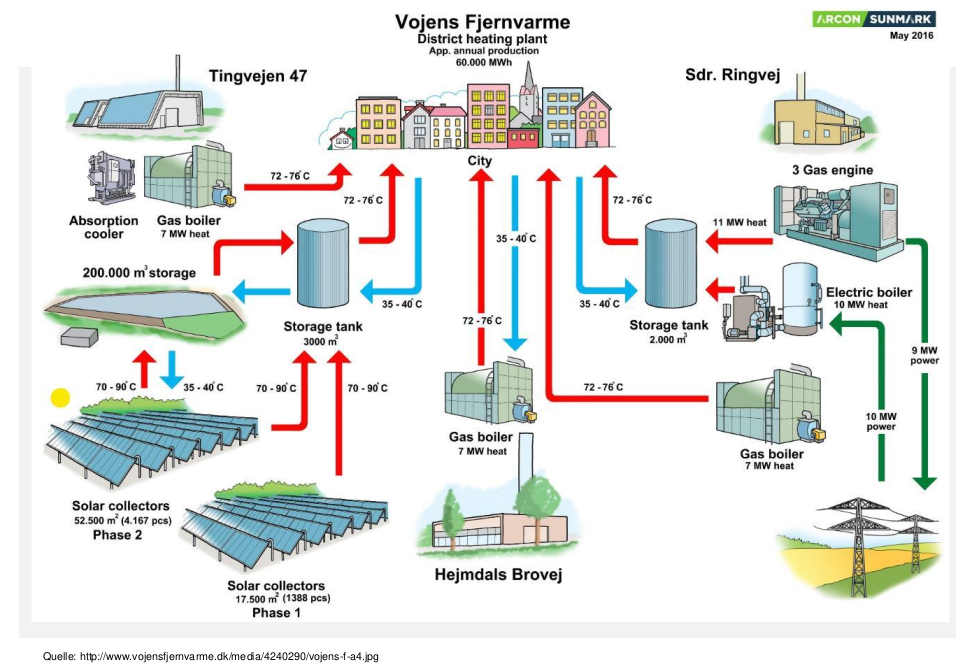
\includegraphics[width=\linewidth]{Medien/own/Vojens_Fernwärme_Wärmeerzeuger.png}
				\caption{Wärmeerzeuger im Fernwärmenetz Vojens \cite[S.40]{wellenbrink_bruegging_2022_waermeleitplanung}}
				\label{fig:Vojens_Fernwärmenetz_Struktur}
			\end{figure}
				
			\begin{table}[H]
				\centering
				\fbox{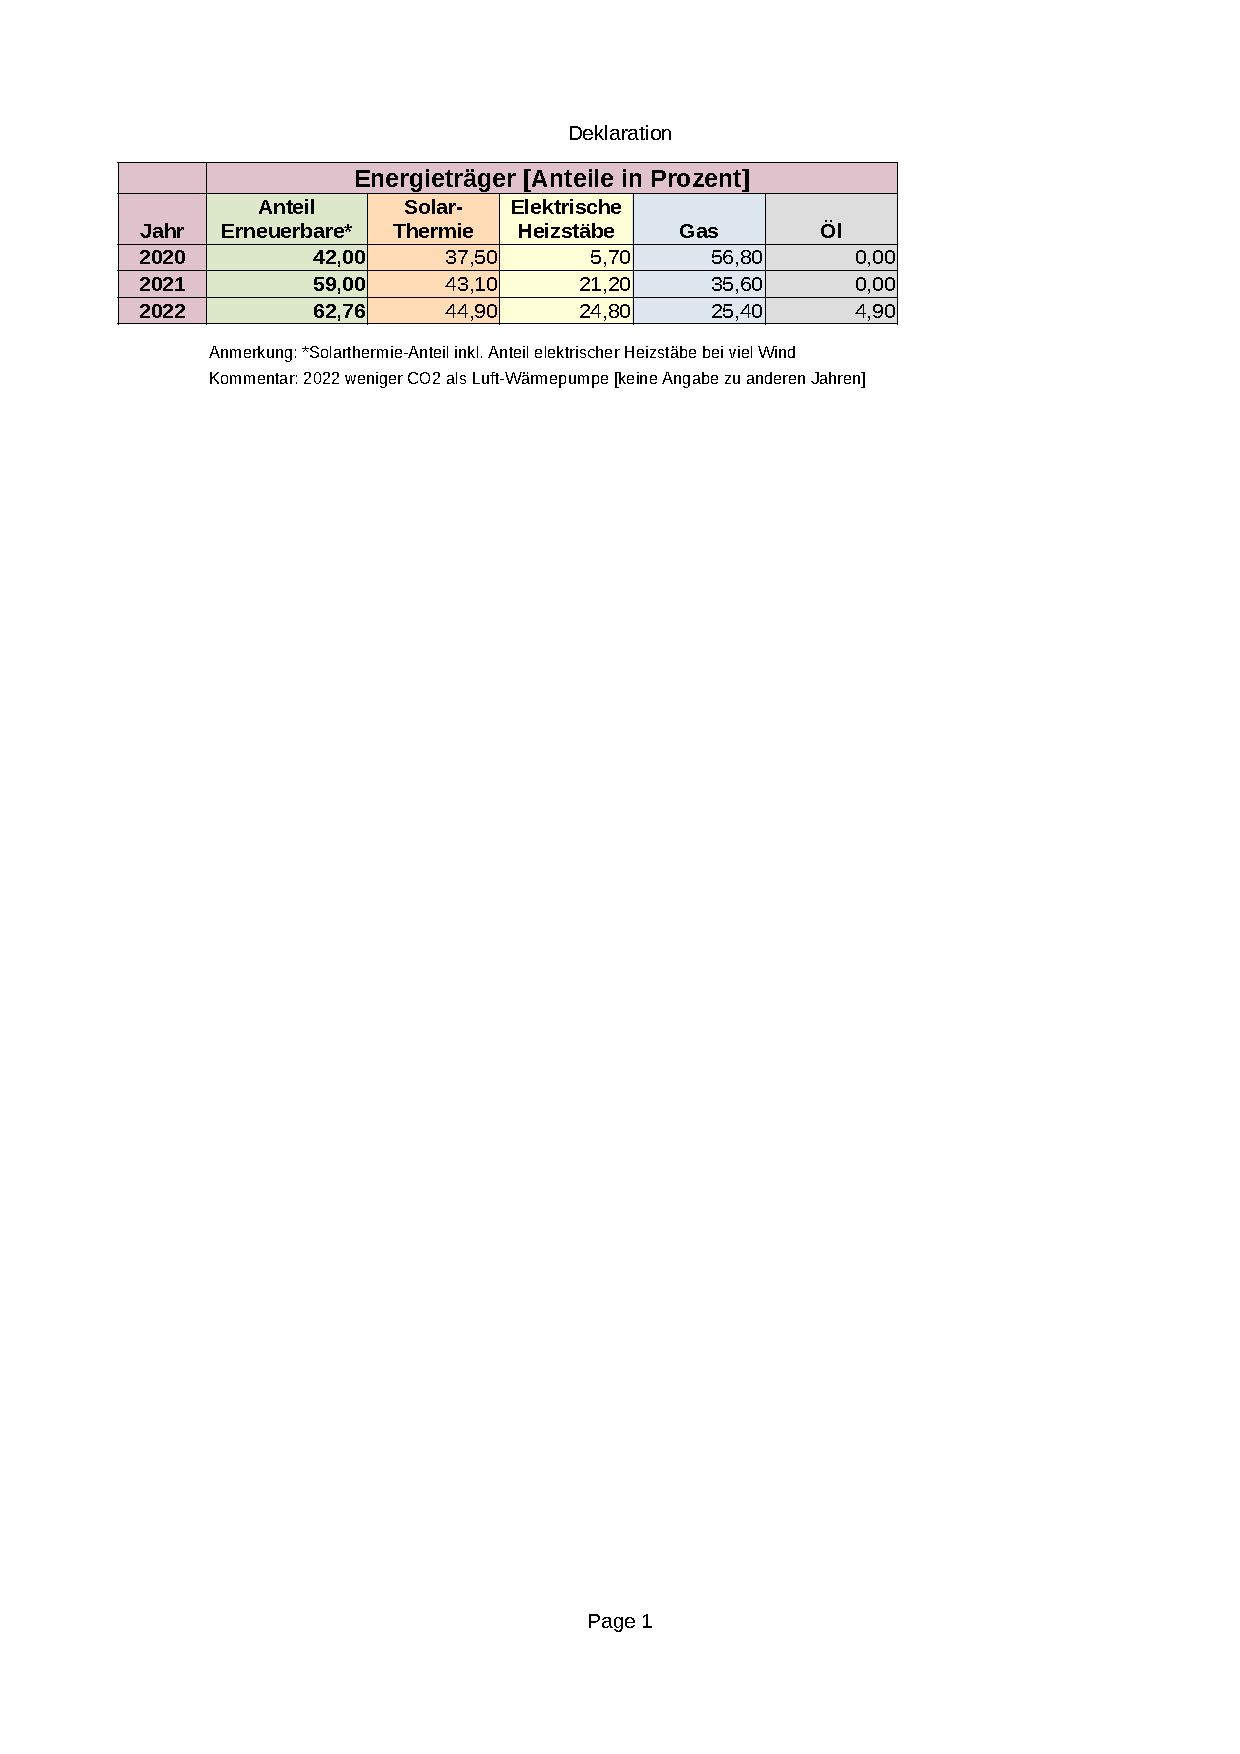
\includegraphics[clip, trim=1.5cm 23cm 4.5cm 2.5cm, width=1.00\textwidth]{Medien/tables/Vojens_Fjernvarme.pdf}}
				\caption{Relative Anteile der Energieträger im Fernwärmenetz Vojen nach Betreiber*innen Deklarationenen 2020, 2021 und 2022 \cite{web_vojens_deklaration}}
				\label{tab:Vojens_Fernwärmenetz}
			\end{table}
			
			Der Wärmeabsatz zwischen 2004/2005 und 2017/2018 betrug zwischen minimal 38.329 MWh (2006/2007) und 49.556 MWh (2010/2011). Absolute Zahlen zu den Jahren danach sind auf der Betreiber*innen-Seite nicht angegeben, allerdings dürften sich diese in einer ähnlichen Größenordnung bewegen. Für die Jahre 2020, 2021 und 2022 hat das Versorgungsunternehmen Deklarationen veröffentlicht mit Angabe der relativen Anteile der einzelnen Energieträgern am Wärme-Mix, welche in \autoref{tab:Vojens_Fernwärmenetz} aufgelistet sind. Der Anteil der Erneuerbaren erreicht durch Nutzung von Solarthermie, Windstrom gespeister elektrischer Boiler und dem Wärmespeicher in den 3 gezeigten Jahren Werte zwischen 42 und 63 \%. Der Anteil von ca. 30 \% aus Gas und Öl im Jahr 2022 soll noch durch eine große Wärmepumpe ersetzt werden.
			
			Auch unter Annahme gleichbleibender absoluter Anteile an Erneuerbaren ergibt eine Witterungsbereinigung mittels Korrekturfaktor aus den Heizgradtagen der besagten 3 Jahre und jenen aus der Referenzperiode 2003 bis 2022 (20 Jahre) ähnliche Anteile an Erneuerbaren. Die jährlichen Heizgradtage in Dänemark im selben Zeitraum betrugen 3019,14 Kd/a (2022), 3263,77 (2021) und 2920,71 (2020) bzw. im Schnitt 3183,21 Kd/a. Daraus ergäben sich nach folgender Rechnung EE-Anteile von 66,17 \% (2022), 56,57 \% (2021) und 45,77 \% (2020). \cite{web_vojens_deklaration} \\ 
			
			$EE_{bereinigt} = \frac{EE_{unbereinigt}}{k} = EE_{unbereinigt} \cdot \frac{HGT_{Durschnitt}}{HGT_{Bezugsjahr}}$
			
			Das Fernwärmenetz Vojen ist bereits jetzt ein Muster-Beispiel für kommunale Wärmeversorgung mit hohem EE-Anteil und besitzt Vorzeige-Charakter mit dem ambitionierten Vorhaben mittels Wärmepumpen vollkommen auf Erneuerbare umzusteigen.\\
			
			\textbf{Weitere Pilotprojekte in Baden-Württemberg in Deutschland}\\
			Die KEA-BW stellt auf ihrer Webseite einige "Best-practice"-Projekte für kommunale Wärmeplanung in Baden-Württemberg vor. Die Versorgungsstruktur der einzelnen Projekte sind dabei sehr individuell auf die jeweiligen lokalen Begebenheiten angepasst. Beispiele ist u.A. das SolarHeatGrid in Ludwigsburg, welches mit einer Kollektorfläche von 14.800 $m^2$ die größte Solarthermie-Anlage in Deutschland im Jahr 2020 darstellte mit einer Wärmeerzeugung von 5.500 MWh/a inkl. 2.000 $m^2$ großem Wasser-Wärmespeicher. Das Wärmenetz in Malsch erzeugt beispielsweise 2.000 MWh/a an Wärme mit einer Kombination aus: Seewasser-Kollektor mit Wärmepumpe, Biogas-BHKW, Holzhackschnitzel-Kessel, Gas-Spitzenlast-Kessel und einem Wärmespeicher. Davon stammen 450 MWh/a aus dem See. \cite{web_kea_bw_waermewende_best_practice}
		
		\subsection{Wärmenetze als Systemdienstleister in integrierten zukunftsfähigen Energiesystemen}
		\label{sec:Grundlagen:Wärmewende_in_D:Wärmenetze_als_Systemdienstleister}
			Wärmenetze können als Schnittstelle zwischen Strom- und Wärmesektor wichtige Systemdienstleistungen übernehmen. Daher wird ihnen zum Beispiel von der Klimaschutz- und Energieagentur Baden-Württemberg GmbH (KEA-BW) in ihrem Positionspapier aus dem Jahr 2014 zur Bedeutung von Wärmenetzen für die Energiewende eine signifikante Rolle für die Dekarbonisierung von Energiesystemen zugeschrieben. \cite{kiezlen_2014_bedeutung_waermenetze_fuer_energiewende} 
			
			Im Leitfaden für kommuale Wärmeplanungen der KEA-BW sind die im Positionspapier aufgelisteten Aufgaben, welche Wärmenetze bedienen können, in etwa wie folgt zusammengefasst \cite[S.~18]{kea_bw_leitfaden_waermeplanung}:
			
			\begin{itemize}
				 \item{Erschließbarmachung lokaler erneuerbarer Energien (Solarthermie, Tiefe Geothermie, Umweltwärme, Biomasse)}
				 \item{Deckung von Bedarfslücken der Stromerzeugung aus Wind und Solar durch bedarfsgerecht betriebene, stromnetzgeführte KWK-Anlagen}
			 	\item{Bereitstellung von Regelleistung durch stromnetzorientiertes Temperatur-Toleranz-nutzendes Demand-side-Management z.B. beim Einsatz von Wärmepumpen}
				 \item{Flexibilitätszugewinn im Wärme- und Stromsektor durch Einbindung großer thermischer Speicher}
				 \item{Erhöhung der Systemeffizienz durch Nutzbarmachung von Abwärme}
				 \item{Instrument sein mit Steuerungsfunktion für Kommunen z.B. um THG-Emissionen zu vermeiden}
			\end{itemize}
		
			Diese Eigenschaften von Wärmenetzen machen kommunale Wärmeplanungen zu einem wichtigen Instrument im Zuge der Energiewende, um klimafreundlich und ressourcenschonend eine zukunftssichere und ökonomisch-tragfähige Wärmeversorgung zu gewährleisten.  
		
	\section{Wärmeplanung Prinzipien}
	\label{sec:Grundlagen:Wärmeplanung_Prinzipien}
			Wärmepläne verfolgen das Ziel eine Status-Quo-Analyse zur Wärmestruktur im jeweils untersuchten Gebiet zu ermitteln, eine Potentialanalyse für vorhandene Ausbaupotentiale für die Wärmeversorgung, eine Formulierung des Zielszenarios und der Umsetzungsstrategie. 
			
			Welche Aufgabenschritte eine Wärmeplanung vorraussetzt und wie diese angegangen werden sowie die Rolle der beteiligten Akteur*innen wird in diesem Kapitel näher beschrieben. 	
			
		\subsection{Prozess der Wärmeplanung}
			Einen guten Überblick über das Vorgehen beim Durchführen von Wärmeplanungen gibt der strategische Leitfaden für kommunale Wärmeplanungen der KEA-BW. Die Beschreibung der einzelnen Prozessschritte in diesem Unterkapitel ist stark an diesen angelehnt. Der Prozess umfasst dabei die folgenden vier Elemente Bestandsanalyse, Potentialanalyse, Aufstellung des Zielszenarios und Wärmewendestrategie. \cite{kea_bw_leitfaden_waermeplanung}
			
			\subsubsection{Bestandsaufnahme}
				In der Bestandsaufnahmen wird der vorhandene Wärmebedarf und -verbrauch sowie die daraus resultierenden THG-Emissionen ermittelt. Darüber hinaus werden Informationen zum Gebäudebestand (Typen und Altersklassen), Versorgungsstruktur inklusive vorhandener Gas- und Wärmenetze, Heizzentralen und Speicher gesammelt. 
				Eine weitere Orientierung für die Bestandsaufnahme gibt auch die Unterteilung der zu erfassenden Daten bezüglich Gemeindestruktur und Energiebilanz.
				
				\textbf{Informationen zur Gemeindestruktur umfassen:}
				\begin{itemize}
					\item{Gebäudebestand (Alter, Nutzungsart), Gebietstyp, Wohndichte}
					\item{Bestehende Wärmenetze, Gasnetze, Lage und Leistung von Heizzentralen sowie KWK-Anlagen und beschlossene Projekte der Wärmeversorgung}
					\item{Bestehendes Glasfasernetz und Ausbaupläne für mögliche gemeinsame Tiefbaumaßnahmen beim Wärmenetzausbau}
				\end{itemize}
		
				\textbf{Energie- und THG-Emissions-Bilanz:}\\
				Für die Ermittlung der Energiebilanz bieten sich zwei Verfahren an:\\
				1) Bottom-Up (Räumlicher aufgelöster Wärmebedarf -> aggregiert für das ganze Gebiet)\\
				2) Top-Down (Gesamter Wärmebedarf -> Aufschlüsselung der räumlichen Verteilung)\\
				
				Die Ermittlung der THG-Emissionen ist wichtig, um realistische Zielszenarien und Transformationspfade zu entwickeln. Die THG-Bilanz leitet sich dann aus dem Wärmeverbrauch und der Zusammensetzung der genutzten Energieträger ab. Zur Veranschaulichung beider Bilanzen bietet sich eine Einteilung nach Sektoren und nach Energieträgern wie folgt an:\\
				- Sektoren: private Haushalte; Gewerbe, Handel und Dienstleistungen (GHD); Industrie; kommunale Einrichtungen\\
				- Energieträger: Erdgas, Heizöl, Erneuerbare, Wärmenetz, Kohle, Sonstige\\
				
				Anmerkung:\\
				- Statistische Abschätzung Verbrauchsdaten: Ungenau, Abweichung (s. Möller, Wiemers 2019, Wärmeplan Flensburg)\\
				- Verbrauchsdaten/Haus: Genau, von Kommunen je nach Bundesland abfragbar\\
				- Verbrauch bei lagerbaren Energieträgern (Heizöl, Kohle, Pellets) nur bedingt aussagekräftig\\
				
			\subsubsection{Potentialanalyse}
				
				In der Potentialanalyse wird das Einsparpotential für Wärmeverbrauche (Raumwärme, Warmwasser, Prozesswärme) ermittelt und die lokal verfügbaren noch ungenutzten Wärmequellen auf ihr erschließbares Potential hin untersucht. Üblich für die Quantifizierung letzterer ist eine Einteilung nach deren Realisierbarkeit. 
				
				\textbf{Potentialklassen von groß nach klein:}
				\begin{itemize}
					\item{Theoretisches Potential: Physikalisch machbar}
					\item{Technisches Potential: Mit Berücksichtigung der Gesetzeslage}  
					\item{Wirtschaftliches Potential: Mit Berücksichtigung der Gesetzeslage und Wirtschaftlichkeit}
					\item{Realistisches Potential}
				\end{itemize}
				
				Die verschiedenen Potentiale sind jeweils Teilmenge des nächst höheren Potentials nach Eingrenzung nach bestimmten Aspekten. Das theoretische Potential umfasst alle theoretisch-technisch möglichen Maßnahmen. Unter Berückschtigung de rechtlichen Rahmenbedingungen ergibt sich daraus das technische Potential. Werden zusätzlich finanzielle Bewertungen nach Kosten- und Gewinnabschätzungen hinzugezogen ergibt sich daraus die Eingrenzung zum ökonomisch (betriebs- oder volks-)wirtschaftlich sinnvollen Potential, dem technisch-wirtschaftlichen Potential. 
				
				Um das realistische Potential für Wärmequellen zu ermitteln wird sukzessiv vorgegangen. Ausgehend vom theoretischen Potential erfolgt die Eingrenzung anhand der Potentialklasseneinteilung. Für die Bestimmung des theoretischen Potentials wird das bestehende Planungs- und Genehmigungsrecht hinzugezogen. Danach werden Annahmen zur technisch wirtschaftlichen Effizienz zur weiteren Eingrenzung getroffen. Ergibt sich kein zielführender Transformationspfad, sind strategische Maßnahmen zu definieren, um neue Potentiale zu Erschließen (z.B. die Ausweisung neuer Flächen) und der Wärmeplan wird iterativ angepasst.
								
				Das betrachtete Gebiet für die Potentialanalyse ist grundsätzlich unabhängig von der Einteilng von Kommunen in Einzelgebiete oder Quartiere und von möglichen Versorgungsgebieten. Diese Vorgehensweise wird vorgenommen, da der Raumbezug im Energiesystem der Zukunft sich dynamisch anhand der Entscheidung für einen Transformationspfad hin zum gewählten Zielszenario ergibt. Mithilfe der Erfassung aller (Ab-)Wärmepotentiale kann die lokale Wärmewendestrategie flexibel und zubaufähig mit Szenarien erarbeitet werden. \cite{kea_bw_leitfaden_waermeplanung}
				
				Die technischen Potentiale lokaler erneuerbarer Energien werden i.d.R. gebietsscharf und Abwärmequellen punktuell erhoben. 
				
				\textbf{Liste zu untersuchender Wärmequellen}
				\begin{itemize}
					\item{\textbf{Abwärme} (z.B. aus Industrieprozessen, Serverfarmen, Fertigungsanlagen, Abwasser)}
					\item{\textbf{Umweltwärme} (z.B. aus Flüssen und Seen)}
					\item{\textbf{PV/Solarthermie} (Freiflächen, Dachflächen)}
					\item{\textbf{Geothermie} (z.B. max. zulässige Bohrtiefe und Wasserschutzgebiete)}
					\item{\textbf{Biomasse} (Nachwachsende Reststoffe und Energiepflanzen, Organische Abfälle, Klärgas, Biogas)}
				\end{itemize}
				
				\textbf{Anmerkungen aus dem Wärmeleitfaden der KEA-BW \cite{kea_bw_leitfaden_waermeplanung}:}\\
				- Deponiegas muss nicht ausgewiesen werden, aufgrund vernachlässigbarer Potentiale\\
			 	- Freiflächen Berücksichtigung ab 2000 $m^2$ (ca. 270 MWh/a)\\
				- Dachflächen Berücksichtigung ab 50 $m^2$ Grundfläche (Für Solarthermie 25\%, für PV 50\% der Grundfläche)\\
			
				Es gibt bestehende Software-Lösungen zur Bilanzierung des Energiebedarfs und der THG-Emissionen nach Sektoren bzw. Energieträgern wie die von der KEA-BW im Leitfaden für kommunale Wärmeplanungen erwähnten Tools (inkl. Herausgeber) \textit{Klimaschutzplaner} (Klimaschutz-Bündnis), \textit{BICO2BW} (KEA-BW) und \textit{ECOSPEED Region} (ECOSPEED AG), welche entweder kostenpflichtig sind oder nur auf Anfrage bei der KEA-BW bereit gestellt werden. 
			
			\subsubsection{Aufstellung Zielszenario}
				
				Für die Aufstellung von Zielszenarien für Wärmeplanungen ergibt sich aus dem Klimaschutzgesetz die Mindestanforderung bis 2045 klimaneutral zu sein. Das bedeutet für die Entwicklung der Verbrauchs- und Versorgungsszenarien, dass die Wärmeversorgung bis 2045 vollständig dekarbonisiert sein muss. Ziele die über diese Vorgaben hinausgehen können ebenfalls Grundlage für die Wärmeplanung sein. \cite{web_gesetze_ksg} \cite{kea_bw_leitfaden_waermeplanung}
				
				Die Mindestanforderungen für die Klimaschutz-Ziele können je nach Landesgesetz auch höher liegen. Beispielsweise sieht das Klimaschutz- und Klimawandelanpassungsgesetz Baden-Württemberg
				(KlimaG BW) in §10 Abs. 1 das Erreichen der Netto-Treibhausgasneutralität bis zum Jahr 2040 vor. Gemäß der Begriffsbestimmung in §2 Abs. 16 ist \frqq Kommunale Wärmeplanung im Sinne dieses Gesetzes [...]ein strategischer Planungsprozess mit dem Ziel einer klimaneutralen kommunalen Wärmeversorgung bis zum Jahr 2040 einschließlich der Aufstellung eines kommunalen Wärmeplans.\flqq \cite{web_gesetze_klimag_bw}
				
				Für nähere Informationen zur Aufstellung von Zielszenarien sei hier auf den Leitfaden für Kommunale Wärmeplanung der KEA-BW verwiesen. \cite{kea_bw_leitfaden_waermeplanung}
				
			\subsubsection{Wärmewendestrategie}
			
				Die Entwicklung einer geeigneten Wärmewendestrategie, um die in den aufgestellten Szenarien gesetzten Ziele zu erreichen, obliegt den Wärmeplanenden. Für nähere Informationen zur Entwicklung einer Wärmewendestrategie sei hier ebenfals auf den Leitfaden der KEA-BW für Kommunale Wärmeplanung verwiesen. \cite{kea_bw_leitfaden_waermeplanung}
			
		\subsection{Akteure, Aktricen, Andere beteiligte}
		
			Neben den Kommunen, welche kommunale Wärmeplanungen durchführen, gibt es eine Vielzahl an Agierende, welche während eines Wärmeplanungsprozesses eine Rolle spielen. Als Schlüsselbeteiligte werden im Paper Wärmewende im Quartier - Hemmnisse bei der Umsetzung am Beispiel energetischer Quartierskonzepte des difu aus dem Jahr 2016 auch private Gebäudeeigentümer*innen, institutionelle Wohnungsunternehmen und Energieversorgungsunternehmen betrachtet. \cite{difu_2016_waermewende_im_quartier_hemmnisse}
						
			Die heterogene Struktur der Beteiligten einer lokalen Wärmewende wird auch im Kurzgutachten Kommunale Wärmeplanung des Umweltbundesamtes von Dezember 2022 erwähnt und dort auf die teils sehr kleinteilige Eigentumsstruktur von Gebäuden zurückgeführt und die Tatsache, dass die Infrastruktur zur Versorgung mit Wärme, Gas und Strom in den Händen unterschiedlicher Betreibenden liegen kann. \cite{uba_2022_kurzgutachten_waermeplanung}
			
			Eine Darstellung des Beteiligten-Spektrums nach difu ist zum Überblick in \autoref{fig:difu_2016_waermewende_lokal_akteurinnen_spektrum} gezeigt. \cite{difu_2016_waermewende_im_quartier_hemmnisse} 
			
			\begin{figure}[H]
				\centering
				\includegraphics[width=1.00\textwidth]{Medien/own/Akteurinnenspektrum_Wärmewende_lokal_difu_2016_Hemmnisse.png}
				\caption{Beteiligten-Spektrum einer lokalen Wärmewende \cite[S.~19]{difu_2016_waermewende_im_quartier_hemmnisse}}
				\label{fig:difu_2016_waermewende_lokal_akteurinnen_spektrum}
			\end{figure}
			
			Sowohl im erwähnten Bericht des difu als auch im Kurzgutachten des UBA wird die Rolle von gesetzgebenden Institutionen wie Bund und Länder vernachlässigt. Erwähnung finden diese z.B. im Abschlussbericht Systemische Herausforderungen der Energiewende des UBA aus dem Jahr 2021. \cite[S.~345]{uba_2021_systemische_herausforderungen_der_energiewende_abschlussbericht}
			
			Im Folgenden soll kurz auf die Rolle einiger als Schlüsselbeteiligte betrachteten eingegangen werden und wie sich diese in ihrer Rolle auf lokale Wärmewenden beziehen.
			%\todo{kürzen!}
			
			Bund und Länder schaffen die gesetzlichen Rahmenbedingungen für Wärmeplanungen. Dazu gehört zum Beispiel auch die Zuweisung von Rechten und Pflichten an Kommunen, Energieversorgungsunternehmen (EVUs) und Netzbetreibende. Mehrere Möglichkeiten der Einflussnahme von Gesetzgebenden für eine klimagerechtere Wärmeversorgung werden zum Beispiel im Policy Paper Wärmewende in Städten gestalten - Empfehlungen für eine sozial-ökologische Transformation der Wärmeversorgung am Beispiel von Berlin aus dem Jahr 2020 genannt. \cite{dunkelberg_2020_waermewende_in_staedten_gestalten}
			
			Energieversorgungsunternehmen, sowohl private als auch kommunale, besitzen zum einen Anlagen zur Erzeugung von Wärme- und/oder Strom und sind damit im Besitz wichtiger Einheiten der Versorgungsinfrastruktur. Zum anderen besitzen sie genaue Verbrauchsdaten aller Kund*innen in ihrem Versorgungsgebiet. Darüber hinaus können sie wichtige Akteur*innen bei der späteren Umsetzung eines Wärmeplans spielen z.B. durch den Planung, Bau und Inbetriebnahme neuer Anlagen. 
			
			Wohnungsunternehmen und private Gebäudeeigentümer*innen obliegt es energetische Sanierungsarbeiten an ihren Gebäuden durchzuführen bzw. durchführen zu lassen, zudem besitzen sie Informationen zur Gebäudestruktur, beispielsweise auch zu bereits durchgeführten oder noch geplanten Modernisierungsmaßnahmen. 
				
					
			%Ggf. in Kooperation mit Zivilgesellschaftlichen Organisationen wie Genossenschaften und Co. ???\\
			
			%Institutionen auf Landesebene wie die KEA-BaWü und das LANUV-NRW: Datenaufbereitung, Forschung, Leitfäden, Ratgeber \\
			
			%Forschungsinstitutionen (Universitäten und co.): Forschung und ggf. in Kooperation mit EVUs/Stadtwerken praktische (Pilot-)Projekte\\
		
		\subsection{Rechtslage in Deutschland}
		\label{sec:Grundlagen:Rechtslage_in_Deutschland}
			Aufgrund des föderalen Charakters der deutschen Bundesrepublik ist die Rechtslage in Deutschland nicht eindeutig und hängt sowohl vom Bundesgesetz als auch den Gesetzen der jeweiligen Ländern ab. Nach Einschätzung der Autor*innen des Policy Papers \frqq Wärmewende in Städten gestalten - Empfehlungen für eine sozial-ökologische Transformation der Wärmeversorgung am Beispiel von Berlin\flqq aus dem Jahr 2020 vom IÖW reichen die \frqq Die zentralen Instrumente und Maßnahmen der Bundesebene [...] bislang nicht für eine Wärmewende im Sinne der Klimaneutralität.\flqq Da auf lokaler Ebene viel für die Wärmeplanung erforderlichen Wissens vorliege, sehen die Autor*innen die kommunale Ebene grundsätzlich als geeignete Umsetungsebene für Wärmeplanungen und heben die Notwendigkeit hervor auf Landesebene einen geeigneten Rechtsrahmen zu schaffen. \cite{dunkelberg_2020_waermewende_in_staedten_gestalten}
			
			Baden-Württemberg hat 2019 im Zuge der Erneuerung des Klimaschutzgesetzes (KlimaG) beschlossen, die größten kreisfreien Städte zu verpflichten bis zum 31.12.2023 Wärmepläne zu erstellen. Eine solche Verpflichtung für Kommunen gibt es in den wenigsten Bundesländern. Zusätzlich gibt es ein landesweites Förderprogramm für die freiwillige kommunale Wärmeplanung für alle Planungskonvois und Gemeinden. Die Möglichkeit der Verpflichtung von Kommunen zu Wärmeplanungen liegt dabei in der Kompetenz der Länder, nicht des Bundes. 
			\cite{uba_2022_kurzgutachten_waermeplanung} \cite{dunkelberg_2020_waermewende_in_staedten_gestalten}
	
			Im KlimaG Baden-Württembergs ist auch die Fördermenge für Kommunen für die entstehenden Mehrkosten geregelt. Kommunen werden zudem ermächtigt gebäudegenaue Verbrauchsdaten zum Beispiel von Energieversorgungsunternehmen und Schornsteinfeger*innen zum Zwecke der Durchführung von Wärmeplanungen zu erheben. Ein kommunaler Wärmeplan in Baden-Württemberg ist nach Erstellung verwaltungsintern verpflichtend und entspricht damit dem Charakter eines Flächennutzungsplans. \cite{web_gesetze_klimag_bw} \cite{kea_bw_leitfaden_waermeplanung}
	
			Bundesweite Vorgaben zur Energieeffizienz an Neubauten und sanierte Bauten und Vorgaben zum Anteil Erneuerbarer Wärmequellen für die genutzte Heiztechnik gemäß Gebäudeenergiegesetz (GEG) wurden bereits in \autoref{sec:Grundlagen:Wärmewende_in_D:Politische_Zielvorhaben} beschrieben.
			
		\subsection{Vergleich mit Dänemark: Rechtslage und Wärmeversorgung}
		\label{sec:Grundlagen:Rechtslage_in_Dänemark}
			In Dänemark sind Kommunen bereits seit 1979 anlässlich der Ölkrise 1973 gesetzlich durch das Wärmeversorgungsgesetz zur Durchführung von Wärmeplanungen verpflichtet. Zudem müssen Kommunen Vorranggebiete für Nah- und Fernwärmenetze festlegen. Die Installation von Öl- oder Gasheizungen in Neubauten ist bereits seit 2013 verboten. Seit 2016 ist auch der Austausch alter fossiler Heizungen gegen neue fossile Heizungen verboten. Fossile Energieträger sind zudem höher besteuert als in Deutschland. \cite{waermewende_daenemark}
			
			Dänemark ist dabei nicht nur gesetzlicher Vorreiter, sondern auch bei der Umsetzung der Wärmewende. Derzeit werden etwa 63 \% der dänischen Haushalte mit Fernwärme versorgt, in Kopenhagen sogar bis zu 98 \%. 68 \% der genutzten Fernwärme stammt dabei aus Kraft-Wärme-Kopplung, 50 \% aus Erneuerbaren Energien. Vom gesamten dänischen Wärmebedarf werden bereits 40 \% durch Erneuerbare Energien gedeckt. \cite{waermewende_daenemark} 
			
	\section{Geoinformationssysteme (GIS)}
	\label{sec:Grundlagen:GIS}
		Geoinformationssysteme (GIS) sind Informationssysteme mit denen laut GIS-Wiki nach Ralf Bill (1994) \frqq raumbezogene Daten digital erfasst und redigiert, gespeichert und reorganisiert, modelliert und analysiert sowie alphanumerisch und graphisch präsentiert werden. \flqq Laut Wikipedia sind GIS Informationssysteme zur \frqq zur Erfassung, Bearbeitung, Organisation, Analyse und Präsentation räumlicher Daten. Geoinformationssysteme umfassen die dazu benötigte Hardware, Software, Daten und Anwendungen.\flqq In manchen Definitionen wird auch die Eigenschaft \frqq rechnergestützt\flqq genannt, welches analoge Karten ausschließt. \cite{web_giswiki_gis}\cite{web_wikipedia_gis}
	
		Die Darstellung verschiedener Geodatensätze in GIS-Anwendungen geschieht in Ebenen (Layer), welche übereinander geschichtet werden. Als Basislayer bieten sich Umgebungskarten an, darüber liegende Layer können Einzelne Objekte bspw. Gebäude oder ähnliches darstellen. 
	
		\subsection{Koordinaten-Bezugssystem}
			Kartographische Darstellungen sind niemals exakt, weil sich eine die Oberfläche eines drei-dimensionalen Körpers nicht zugleich flächen- noch winkeltreu auf einer zwei-dimensionalen Fläche abbilden lässt. Das Ziel von Koordinaten-Bezugs-Systemen (KBS), im englischen auch coordinate reference system (CRS) genannt, ist einen einheitlichen Rahmen zu schaffen, zur präzisen Messung von Raumpunkten und zur konsistente Darstellung dieser als Koordinaten, welche eindeutig die gemessenen Raumpunkte wiedergeben. 
			
			Ein KBS umfasst ein Koordinaten-System, ein Datum, und eine Projektion. Das Koordinatensystem umfasst dabei einen Ursprungspunkt, Axen, welche vom Ursprungspunkt ausgehen und eine Einheit, in welcher Koordinaten gemessen werden. Das Koordinatensystem kann beispielsweise die Form einer Kugel, eines Ellipsoids, z.B. dem Geodätischen Referenzsystem 80 (GRS 80), oder eines Geoids, z.B. dem Earth Gravitational Model 96 (EGM 96) annehmen. Geoide sind drei-dimensionale geometrische Formen mit delliger Oberfläche, salopp gesagt \frqq Kartoffeln\flqq, mit globusähnlicher Form. \cite{web_wikipedia_crs}
			
			Ein KBS eignet sich je nach gewähltem Koordinatensystem, Datum und Projektion eher für eine möglichst flächentreue oder eher winkeltreue Abbildung, zudem sind die Abweichungen abhängig von der abzubildenden Region auf dem Globus. Veranschaulichen lässt sich dies, durch Verschiebung (Datums-Änderung) und Verformung eines Referenz-Ellipsoids (Koordinatensystem-Änderung) in Bezug zum Globus. Je näher die Referenz-Oberfläche an der Globus-Oberfläche der gewählten Region liegt, desto genauer die Abbildung. 
			
			Die Projektion beinhaltet Abbildungsvorschriften, also Definitionen zur Umrechnung der Referenz-Koordinaten in Karten-Koordinaten. Geokoordinaten lassen sich so auch von einem KBS in ein anderes KBS projezieren bzw. umrechnen. Eine mögliche Projektion ist beispielsweise Lamberts winkeltreue Kegelprojektion oder die ebenfalls auf Johann Heinrich Lambert zurückgehende Flächentreue Azimutalprojektion (englisch Lamberts Azimutal Equal Area Projection). Erstere bildet eine Kugeloberfläche flächentreu auf die Mantelfläche eines Kegels ab, letztere bildet eine Kugeloberfläche flächentreu auf eine Scheibe ab. \cite{web_wikipedia_lambert_conformal_cone_projection}\cite{web_wikipedia_lambert_azimutal_equal_area_projection}
			
			Als einheitliche Codierung für die allermeisten der weltweit genutzten KBS werden von allen gängigen GIS-Software EPSG-Codes unterstützt. Der EPSG-Datensatz stammt ursprünglich von der namensgebenden European Petroleum Survey Group Geodesy (EPSG), und wird inzwischen vom Geodesy Subcommittee des Geomatics Committee der International Association of Oil \& Gas Producers (IOGP) gepflegt. \cite{web_epsg}
			
		\subsection{QGIS}
			% Allgemein
			QGIS ist ein freie GIS-Software, die unter der GNU General Public Licence (GPL) lizensiert wurde. Das Projekt wurde 2002 gegründet und wird bis heute aktiv fortgeführt. QGIS läuft auf einer Vielzahl an Betriebssystemen, darunter die meisten Unix und unixähnlichen Betriebssysteme (Linux), Windows und macOS. \cite{web_qgis}\cite{web_qgis_docs}
			
			% Features
			Von QGIS gibt es mehrere Anwendung, zum einen die Desktop-Version mit Graphical User Interface (GUI) zur offline-Nutzung, welche auch im Zuge dieser Arbeit verwendet wurde. Zum anderen gibt es noch eine Server- und eine Web-Client-Version zur online-Nutzung und darüber hinaus noch eine mobile Anwendung für Android, iOS und Windows. \cite{web_qgis}
			
			QGIS ist mit einer Vielzahl an Dateiformaten für Geodaten kompatibel. Neben gängigen GIS-Anwendungs-Features verfügt QGIS auch über eine Python-Schnittstelle und eine integrierte Python-Konsole. \cite{web_qgis_docs}
				
		\subsection{Datentypen und Dateiformate}
			% Raster und Vektor
			Geodatentypen lassen sich prinzipiell in raster- und vektorbasiert unterscheiden. Rasterbasierte Geodaten sind Rastergrafiken (Pixelgrafiken), beispielsweise Satellitenfotos mit Geokoordinaten. Hierbei wird die Auflösung die Anzahl der Pixel bestimmt. Im Gegensatz dazu werden in vektorbasierten Geodatensätzen Objekte als Vektografiken also geometrisch definiert, z.B. als Punkte, Linien oder Polygone, denen Geokoordinaten zugewiesen werden. Die Auflösung wird hier bei Polygonzügen (Mehr-Punkt-Strecken und Vielecke) nur durch die Anzahl der Stützpunkte definiert, ist abgesehen davon aber in der Darstellung beliebig skalierbar.
			
			% Formate
			Die verschiedenen Dateiformate bringen unterschiedliche Vor- und Nachteile mit sich bezüglich Kompatibilität, Speicherplatzbedarf und Geschwindigkeit beim Einlesen in GIS-Software. Zudem lassen sich freie und proprietäre Formate unterscheiden. Ein mögliches Raster-Format ist z.B. GeoTIFF. Mögliche Vektor-Formate sind unter Anderem ESRI Shapefiles (kurz Shapefile), GeoJSON, OGC GeoPackage, FlatGeobuf, OGC GML, SpatialLite, OGC KML (keyhole-markup-language), CSV (z.B. mit WKT) und viele mehr.\cite{web_qgis_docs} 
			
			% Vorteil Vektor
			Der große Vorteil vektorbasierter Geodaten jedweden Formats ist die Verknüpfbarkeit von geometrischer Figuren (bswp. Hausumringen) mit anderen Daten, welche diesen als Attribute zugewiesen werden (bspw. Baualtersklasse) und deren besserer Wartbarkeit.  
			
			% Datentypen neben Geodatentypen
			Neben den Geodatentypen gibt es noch GIS-Software-spezifsche Datentypen wie Projektdateien, Styledateien und weitere, in denen beispielsweise Einstellungen gespeichert werden. In QGIS werden Layer-Styledefinitionen beispielsweise im .xml-Format als .qml-Dateien verwendet. In diesen wird definiert, welche Objekte einer Vektorgraphik wie dargestellt werden. Regelbasierte Darstellungsformen ermöglichen eine differenzierte Darstellung von Geometrieobjekten anhand bestimmter Attributswerte, wahlweise in Abhängigkeit von gesetzten Maßstabsgrenzen, dazu gehört auch eine optionale Beschriftungen von Objekten anhand eines Attributswert, z.B. Ortsnamen, Straßennamen und Flächenbezeichnungen. 
			
			\subsubsection{ESRI Shapefiles: Vorteile, Nachteile und Alternativen}
				% Shapefiles Aufbau
				Bei den im Zuge dieser Arbeit betrachteten Datensätzen lag ein Großteil der vektorbasierten Daten als Shapefiles vor. Diese sind laut Jachym Cepickys Plädoyer \textit{Switch from Shapefile} (2017) das üblichste vektorbasierte Format. Der Standard für Shapefiles stammt aus dem 1990er Jahren. Ein Shapefile besteht dabei aus mehreren Dateien. Essentiell ist eine .shp-Datei mit den Geometriedaten, eine .dbf-Datei mit den Sachdaten (Attributstabelle) im dBASE-Format und eine .shx-Datei mit Indizes zur Verknüpfung von Geometrie- und Sachdaten. \cite{web_shapefiles_must_die_cepicky}\cite{esri_shapefile_technical_description}
				
				% dbase limitations: fieldname 32 bytes ( ? -> 10 letters ? ) neuere dbase version
				% https://www.dbase.com/Knowledgebase/INT/db7_file_fmt.htm
				
				% Nachteile Shape Files
				Cepicky nennt in seinem Plädoyer mehrere gravierende Nachteile von Shapefiles. Z.B. sind Attributnamen auf 10 Zeichen begrenzt. Diese werden bei Konvertierung i.d.R. automatisch abgeschnitten, was zu kryptischen Bezeichnungen führen kann. Zudem ist die Definition eines KBS optional und die Dateigröße ist auf 2 GB begrenzt. \cite{web_shapefiles_must_die_cepicky} 
				
				Eine vielversprechende Alternative zu Shapefiles ist das offene Format OGC Geopackage. Dieses wird auch von Cepicky als Alternative genannt und für dieses plädiert auch Simon Baier in seinem Blogpost \textit{Why you should use GeoPackage instead of Shapefile}. Seit Version 3 von QGIS ist OGC GeoPackage auch QGIS Standard-Vektorformat (ehemals Shapefile). Aus diesem Grund wird in dieser Arbeit standardmäßig OGC Geopackage als Speicherformat gewählt. Optional wird versucht Daten auch im Shapefile-Format zu speichern, um eine möglichst große Kompatibilität verschiedener GIS-Software-Applikationen zu erreichen. \cite{web_geopackage_vs_shapefile_blog_simon}\cite{web_qgis_docs}
				
			%csv-Files:\\
			%	Well-known text representation of geometry (WKT) ist eine Spezifikation zur alphanumerischen Darstellung von Objektgeometrien und Teil der \textit{Simple Feature Access} Spezifikation des Open \textit{Geospatial Consortium}.\\
						
			\subsubsection{Beispiel GIS-Web-Anwendung Energieatlas NRW}
				% Allgemein
				Als Beispiel einer GIS-Web-Anwendung dient hier der \textit{Energieatlas NRW} des LANUV. Dieser stellt \frqq umfangreiche Informationen zur Energiewende in Nordrhein-Westfalen zur Verfügung. In den Themenkarten sind landesweit verfügbare Planungsdaten veröffentlicht.\flqq Unter dem Reiter Karten finden sich die Themenkarten \textit{Biomassepotential}, \textit{Planung Wind}, \textit{Rheinisches Revier}, \textit{Solarkataster}, \textit{Strom Bestand} und \textit{Wärmekataster}. \cite{web_energieatlas}
				
				% Wärmekataster
				\autoref{fig:energieatlas_waermekataster} zeigt exemplarisch einige Darstellungsmöglichkeiten der Themenkarte \textit{Wärmekataster} aus dem Energieatlas NRW, wie sie im Zuge von Wärmeplanungen genutzt werden können. Die gezeigten Wärmeliniendichte stammt aus dem Raumwärmebedarfsmodell des LANUV, die Daten für Heiztypen je Baublock sind abgeleitet aus den Daten des Zensus 2011. Die Standorte für Wärmequellen und KWK-Potentiale stammen aus einer Studie des LANUV. Die Daten zum Modernisierungspotential und die Realisierungschancen für energetische Sanierungen stammen aus Schätzungen des LANUV. \cite{web_energieatlas}
				
				\begin{figure}[h]
					\centering
					\subfloat[Subfigure 1 list of figures text][Wärmenetzen, Wärmeliniendichte (1:1000)]{
						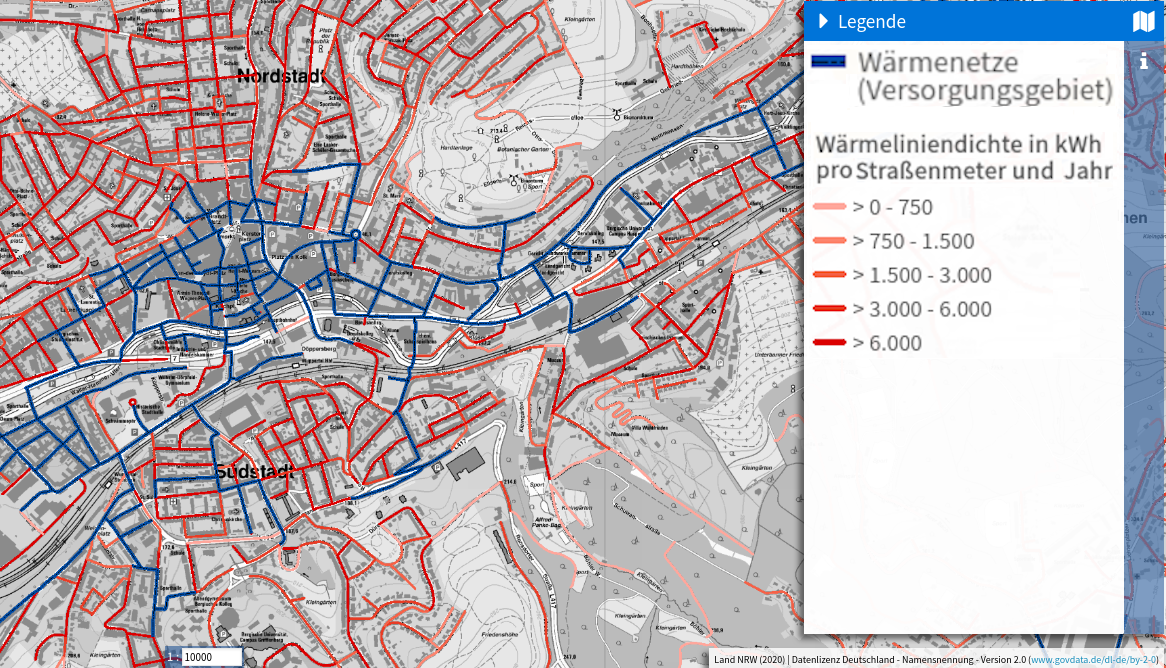
\includegraphics[width=0.45\textwidth]{Medien/own/energieatlas/energieatlas_wärmekataster_netze_wärmeliniendichte.png}
						\label{fig:subfig1}}
					\subfloat[Subfigure 2 list of figures text][Anteil Fernwärme je Baublock (1:1000)]{
						\includegraphics[width=0.45\textwidth]{Medien/own/energieatlas/energieatlas_wärmekataster_baublockebene_anteil_fernwärme.png}
						\label{fig:subfig2}}
					\qquad
					\subfloat[Subfigure 3 list of figures text][Anteil Gasheizungen je Baublock (1:1000)]{
						\includegraphics[width=0.45\textwidth]{Medien/own/energieatlas/energieatlas_wärmekataster_baublockebene_anteil_gasheizungen.png}
						\label{fig:subfig3}}
					\subfloat[Subfigure 4 list of figures text][Anteil Ölheizungen je Baublock (1:1000)]{
						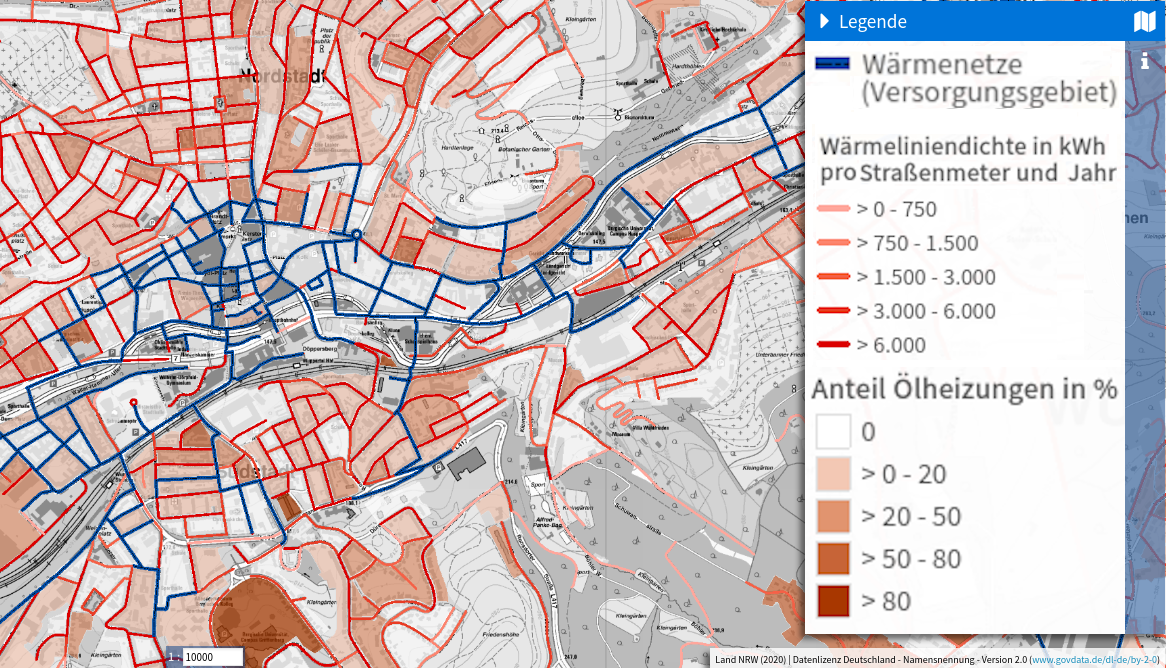
\includegraphics[width=0.45\textwidth]{Medien/own/energieatlas/energieatlas_wärmekataster_baublockebene_anteil_ölheizungen.png}
						\label{fig:subfig4}}
					\qquad
					\subfloat[Subfigure 1 list of figures text][Wärmebedarf je 100 x 100 $m^2$ (1:1000)]{
						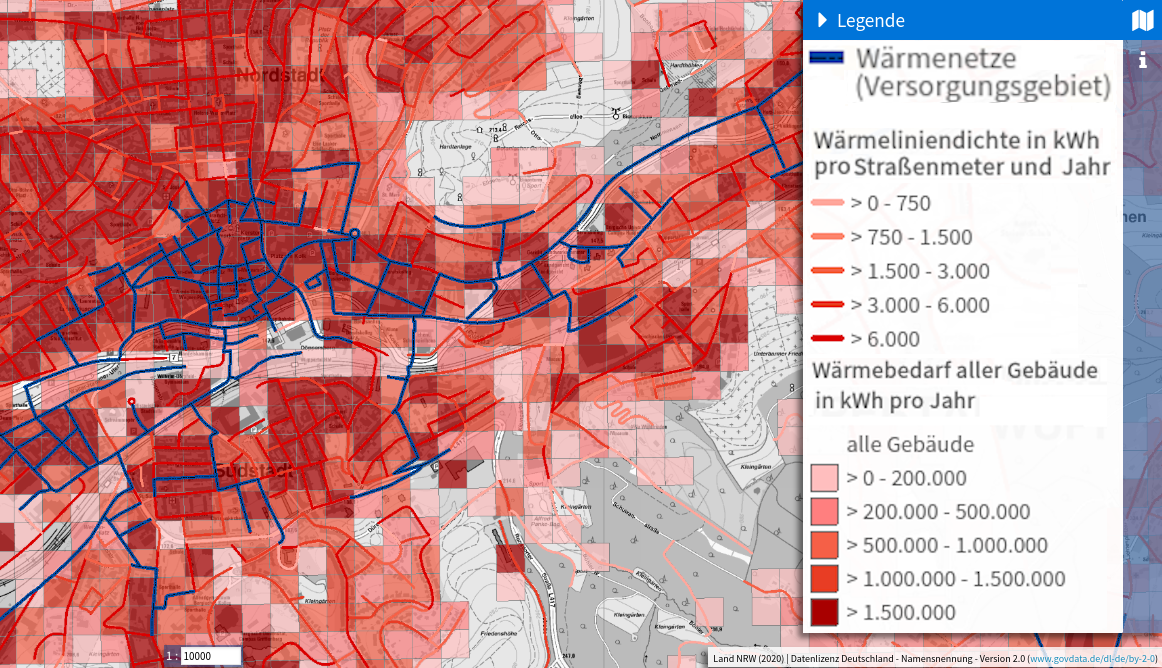
\includegraphics[width=0.45\textwidth]{Medien/own/energieatlas/energieatlas_wärmekataster_wärmebedarf_alle_gebäude.png}
						\label{fig:subfig5}}
					\subfloat[Subfigure 2 list of figures text][Wärmequellen (Energieträger und Standorte), KWK-Wärmepotential je PLZ (1:4500)]{
						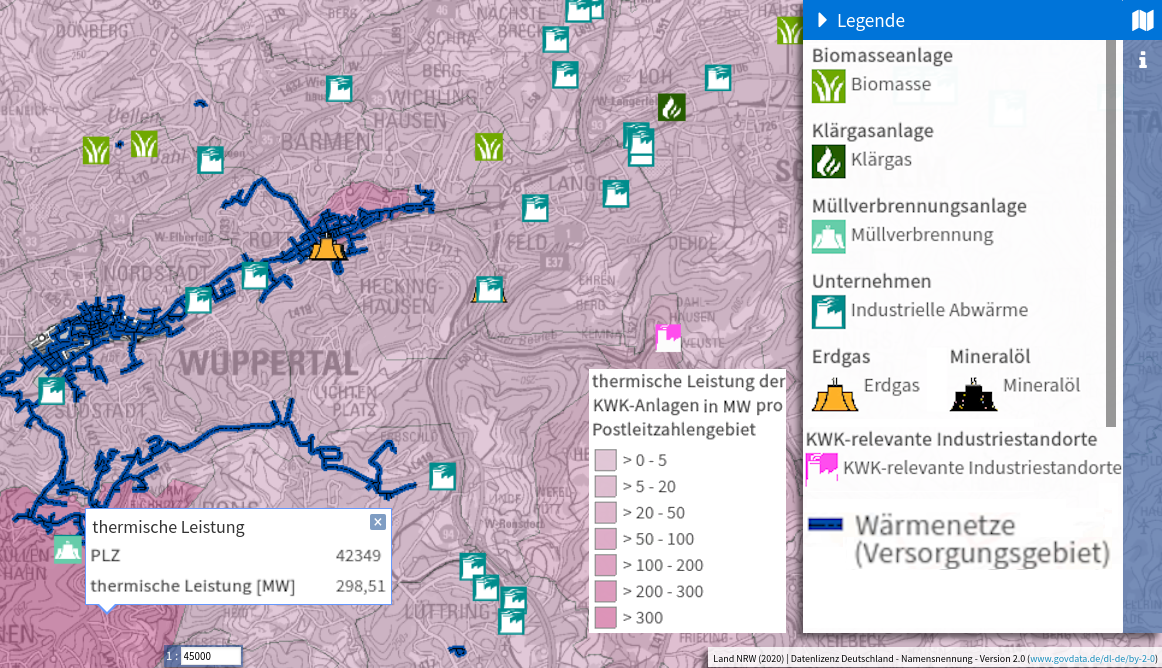
\includegraphics[width=0.45\textwidth]{Medien/own/energieatlas/energieatlas_wärmekataster_wärmequellen_kwk_therm_leistung_je_plz.png}
						\label{fig:subfig6}}
					\qquad
					\subfloat[Subfigure 3 list of figures text][Energetische Gebäudesanierung je Baublock, Modernisierungspotential (1:1000)]{
						\includegraphics[width=0.45\textwidth]{Medien/own/energieatlas/energieatlas_wärmekataster_baublockebene_modernisierungspotential.png}
						\label{fig:subfig7}}
					\subfloat[Subfigure 4 list of figures text][Energetische Gebäudesanierung je Baublock, Realisierschancen (1:1000)]{
						\includegraphics[width=0.45\textwidth]{Medien/own/energieatlas/energieatlas_wärmekataster_baublockebene_realisierungschance_energ_geb_sani.png}
						\label{fig:subfig8}}
					\caption{Energieatlas NRW - Wärmekataster: Eigene Darstellungen, Legende editiert \cite{web_energieatlas}}
					\label{fig:energieatlas_waermekataster}
				\end{figure}
				
				% Solarkataster
				In der Themenkarte \textit{Solarkataster} des \textit{Energieatlas NRW} sind unter Anderem geeignete Frei- und Dachflächen für PV bzw. Solarthermie gezeigt. Geeignete Dachflächen für PV, die keiner Prüfung durch ein Fachunternehmen zur Eignung bedürfen, werden farblich nach Ausrichtung (Flach, Nord, Ost, Süd, West) differenziert markiert. PV-Eignungsflächen lassen sich nach EEG 2021 und nach EG 2023 anzeigen. Zudem enthalten sind Daten zur Globalstrahlung, Strahlungsintensität und Sonnenscheindauer. \cite{web_energieatlas}
				
				% Biomassepotential
				Die Themenkarte \textit{Biomassepotential} des \textit{Energieatlas NRW} zeigt Biomassepotentiale aus der Potentialstudie des LANUV für Strom oder Wärme aufgeteilt nach verschiedenen Szenarien (Minimum, Leit, Maximum) und Sektoren (Landwirtschaft, Forstwirtschaft, Abfallwirtschaft, gesamt). Die Daten werden räumlich nur für ganz NRW aggregiert dargestellt. \cite{web_energieatlas}
				% Eine Stichprobe (Wuppertal, Campus Freudenberg) zeigt, dass bestehende PV-Anlagen nicht gezeigt werden.
				
				% Andere Gis-Web-Anwendungen
				Weitere Beispiele für GIS-Web-Anwendungen sind zum Beispiel der \textit{Zensusatlas} des Zensus 2011 von den Statistischen Ämtern des Bundes und der Länder (destatis) \cite{web_zensusatlas} und die interaktive Karte \textit{Geothermie in NRW - Standortcheck} des Geologischen Dienstes NRW \cite{web_geothermie_standortcheck_nrw}. 
	